\documentclass[german,version-2020-11]{uzl-thesis}


% Copy this file as a template for your thesis. You will have to take
% action at all places marked by
%
% !!!!!!!!!!!!!!!!!!!!!!!!!!!!!!!!!!
% !!! Your action is needed here !!!
% !!!!!!!!!!!!!!!!!!!!!!!!!!!!!!!!!!
%
% The first place your action is needed is the first line of this
% document:
%
%
% Language of the thesis:
%
% You must use either 'german' or 'english' above, depending on the
% language used in the main text. This will automatically setup a lot
% of things in the background.
%
%
% Version of the class:
%
% You must specify which version of the thesis class is to be
% used. This is important in case the class style changes in later
% years, but we still want an older thesis to look the same, even when
% things are changed in the class.
%
% Do not change or remove the version-xxxx key.
%
%
% Text encoding:
%
% Your thesis *must* be encoded in utf8 (unicode), which is the
% default in most editors these days. Do *not* change this to latin8.



%%%
%
% Main setup:
%
%%%
%
% You must use the \UzLThesisSetup command to specify numerous things
% about your thesis. This includes the entries on the title page, the 
% abstracts, and the bibliography style. You do so by specifying
% so-called "values" for so-called "keys". For instance, 
% for the key "Autor" you must provide your name as the value. You do
% so by writing 'Autor = {Max Mustermann}', that is, the value is put
% into curly braces. You can use the \UzLThesisSetup command
% repeatedly and the order in which you provide the keys is not
% important. 
%
% Everything shown on the title page must be in German -- even
% if the thesis is written in English! Just insert German text for
% German keys and English text for English keys (like 'Abstract' needs
% English text, while 'Zusammenfassung' needs German text).

\UzLThesisSetup{
  %
  % !!!!!!!!!!!!!!!!!!!!!!!!!!!!!!!!!!
  % !!! Your action is needed here !!!
  % !!!!!!!!!!!!!!!!!!!!!!!!!!!!!!!!!!
  %
  % First, specify the institut or clinic at which the thesis was
  % written. You get the logo file from them (make sure it has the
  % correct size, namely the same as the example). If they do not have
  % a logo, the university's default logo is used.
  %
  % The 'verfasst' gets two arguments. Change the first to {an der}
  % for clinics, as in 'Verfasst = {an der}{Medizinischen Klinik I}'
  %
  Logo-Dateiname        = {uzl-thesis-logo-itcs.pdf},
  Verfasst              = {am}{Institut für Theoretische Informatik},
  %
  % The titles:
  %
  Titel auf Deutsch     = {
    Kollaboratives, cloud-basiertes Simulationstool für Schwarmrobotik
  }, 
  Titel auf Englisch    = {
    Collaborative cloud-based Simulation Tool for Swarm Robotics
  },
  %
  % Author and supervisor:
  % 
  % Note that the 'Betreuer' or 'Betreuerin' is the supervisor, that
  % is, the professor who officially supervises the thesis. If there
  % is also an assistent of the professor who helped (typically a
  % lot), use 'Mit Unterstützung von' to thank that person. If the
  % thesis was mainly written 'externally' at some company or another
  % institute, point this out using 'Weitere Unterstützung'. 
  % 
  % For your own name, do *not* add things like "BSc" or "BSc
  % cand.". For the supervisor, you should normally include
  % "Prof. Dr." or "PD Dr." (ask your supervisor, what is
  % appropriate), but nothing more (so no
  % "Univ.-Prof. Dr. Dr. h.c. mult." unless your supervisor insists).  
  %
  Autor                 = {Patrick Ugwu},
  Betreuerin            = {Dr. Javad Ghofrani},
  % 
  % Optional: Supporting persons and institutions. The text should be
  % in German, even for an English thesis.
  %
  %Mit Unterstützung von = {Harry Hilfreich},
  % 
  %   Weitere Unterstützung = {
  %     Die Arbeit ist im Rahmen einer Tätigkeit bei der Firma Muster GmbH
  %     entstanden.
  %   },
  %
  %
  % Your Degree Programm (Studiengang)
  %
  % Specify 'Bachelorarbeit' or 'Masterarbeit' and the degree
  % programme. Make sure the name of programme is correct and not
  % some abbreviation or some incorrect variant. For instance:
  % 'Medizinische Ingenierwissenschaft', but not 'MIW';
  % 'Medizinische Informatik', but not 'Medizin-Informatik';
  % 'Informatik', but not 'Informatik (SSE)'.
  %
  % Use German names for German programmes and English names for
  % English ones, so 'Infection Biology', not 'Infektionsbiologie'. 
  % For programmes that have a German bachelor and an English master,
  % use the German name for a bachelor thesis and the English name for
  % the master thesis.
  %
  Bachelorarbeit,
  Studiengang           = {Robotik und autonome Systeme},
  %
  % Date on which the thesis is turned in German, formatted the
  % traditional German way:
  %
  Datum                 = {6. Juli 2024},
  %
  % The English abstract. You must always provide abstracts in German
  % and in English. 
  %
  Abstract              = {
    This bachelor's thesis examines the integration of online collaborative features into robot simulation. 
    The aim of the study is to investigate the feasibility and benefits of a collaborative online tool in the field of swarm robotics simulation. 
    For this purpose, the online simulation tool CollabSim was developed and evaluated through a user test. 
    The impact of using this tool on the simulation process was examined in comparison to traditional simulation methods. 
    The results demonstrate the potential and feasibility of this approach to enhance the effectiveness in creating simulations. 
    The thesis concludes by noting that CollabSim represents a promising prototype. 
    However, it also highlights the need for further research to explore specific advantages and challenges in depth.
  },
  Zusammenfassung       = {
    Diese Bachelorarbeit untersucht die Integration kollaborativer online Funktionen in die Robotersimulation. 
    Ziel der Arbeit ist es, die Machbarkeit und den Nutzen eines kollaborativen, webbasierten Werkzeuges zur Simulation im Bereich der Schwarmrobotik zu untersuchen. 
    Hierfür wurde der Simulator CollabSim entwickelt und mittels eines Nutzertests evaluiert. 
    Dabei wurden die Auswirkungen der Nutzung dieses Werkzeugs auf den Simulationsprozess im Vergleich zu traditionellen Simulationsmethoden untersucht. 
    Die Ergebnisse zeigen das Potenzial und die Machbarkeit dieses Ansatzes zur Verbesserung der Effektivität bei der Erstellung von Simulationen. 
    Die Arbeit schließt mit der Feststellung, dass CollabSim einen vielversprechenden Prototypen darstellt. 
    Dennoch wird aufgezeigt, dass weitere Forschung erforderlich ist, um spezifische Vorteile und Herausforderungen weiter zu untersuchen.
  },
  %
  % Optional: 'Danksagungen' (German) or 'Acknowledgements'
  % (English). Both keys are optional and both have the same effect of
  % adding an acknowledgements text after the abstracts and before the
  % table of contents.
  %
  %Acknowledgements      = {
  %  This is the place 
  %},
  % Bibliography style: Choose between
  % 
  % 'Alphabetische Bibliographie'
  % for all degree programmes in the natural sciences 
  % 
  % 'Numerische Bibliographie'
  % alternative for all other degree programmes
  % 
  % Either will load biblatex and setup the citation methods and the
  % bibliography styles correctly. You should not mess with them.
  % 
  Alphabetische Bibliographie,
  % Alternatively:
  % Numerische Bibliographie
}




%%%%%%%%%%%%%%%%%%%%
%
% Styling the thesis
%
%%%%%%%%%%%%%%%%%%%%
%
% Creating a visually pleasing layout and choosing fonts is not
% easy. Furthermore, different people have different preferences. Of
% course, for the University of Lübeck, the dean of studies could just
% force everyone to use one specific layout and font, but that seems a
% bit drastic and, also, it seems nice that thesis by different people
% have an individual style even though they all stick to the same
% overall structure.
%
% For these reasons, I (Till Tantau) have spend quite some time on
% designing a flexible layout and styling mechanism for theses.
%
% Basically, the overall structure of the thesis is fixed by the
% thesis class and so are many structural elements. For instance, you
% cannot change the order in which the abstract and table of contents
% are shown, you cannot move the bibliography elsewhere, indeed, the
% bibliography style is also fixed. Likewise, the text on the title
% page is fixed.
%
% Although many things are fixed, you *can* change several other
% things. For instance, you can change the font used for the main
% text, you can change which font is used for titles and headings or
% you can change whether titles and headlines are centered or flushed
% left.
%
% There are many LaTeX packages for changing such things. You are
% kindly asked *not to use them*. Rather, use (only) the options
% offered by the thesis class. All possible choices and combinations
% there have been tested by me and produce nice results; what happens
% with other packages no one knows and might no longer conform to what
% is expected by the university. As you will see, you still have a
% lot of options.
%
%
% Technical note: All styling is done via the command
%
% \UzLStyle{...}
%
% where ... is a key-value list just as for \UzLThesisSetup. The
% difference is just that everything having to do with styling as
% controlled by \UzLStyle, while the more “formal” setup keys are
% controlled by \UzLThesisSetup.
%
%%%
%
% Designs
%
%
% A \emph{design} is a whole set of font and layout options bundled
% together. They have been chosen in such a way that a visually
% pleasing “overall appearance” results.
%
%
% \UzLStyle{computer modern oldschool design}
%
% The look of this design mimics the “classical” way a paper or report
% created with \LaTeX\ looks like: The Computer Modern font is used,
% bold face fonts are used for headlines, only black and white are
% used as colors. This design reminds me of older scientific
% documents, especially from the computer science community where
% \LaTeX\ was used very early.
%
%
% \UzLStyle{computer modern basic design}
%
% A slightly less “oldschool” version of the previous design. It is
% still a classic design in the sense that it uses the Computer Modern
% font and that it still has this “good old \LaTeX” look, but some
% more modern aspects (like colors!) have been added.
%
% Note that this design uses Myriad for the title page (one of the
% “modern aspect”), which means that his font must be installed.
%
%
% \UzLStyle{computer modern scholary design}
%
% In my opinion, this is the ultimate “scholary design”: The thesis
% will look like it has been typeset by hand some 150 years ago and
% then printed by a university press. There is really nothing “modern”
% about it and the word in the name of the design is just part of the
% name of the “Computer Modern” font.
%
%
% \UzLStyle{pagella basic design}
%
% A, well, basic design that uses the Pagella font rather than the
% Computer Modern font. Especially the bold face version of this font
% looks nicer than the Computer Modern counterpart. Also, Pagella,
% while still having a “bookish” look, still feels a bit fresher than
% Computer Modern. 
%
%
% \UzLStyle{pagella centered design}
%
% A variant of the basic Pagella design that centers all
% headlines. A nice alternative to the basic version.
%
%
% \UzLStyle{pagella contrast design}
%
% This design tries to create some visual friction by contrasting the
% sans serif headline font (in bold!) with the main text. I find it a
% visually very interesting combination.
%
%
% \UzLStyle{alegrya basic design}
%
% The third variant of the basic design, this time using the Alegrya
% font. 
%
%
% \UzLStyle{alegrya scholary design}
%
% The Alegrya version of the previous “scholary” design. Unlike the
% Computer Modern version, this design does not look old, but more
% fresh -- while still creating the impression that the text must be
% about a very scientific subject. 
%
%
% \UzLStyle{alegrya stylish design}
%
% The design is quite similar to the scholary version for the Alegrya
% font, but with even more modern additions. “Stylish” is the word
% that comes to my mind.
%
%
\UzLStyle{alegrya modern design}
%
% A design that uses the sans serif version of the Alegrya font for
% the headlines. This is a nice modern overall design.
%
%%%




%%%%%%%%
%
% Now, include the package you need here using \usepackage. 
%
% However, many standard packages are already loaded by the class:
%
% amsmath, amssymb, amsthm, babel, biblatex, csquotes, etoolbox,
% filecontents, fontspec, geometry, hyperref, tikz (with libraries
% arrows.meta, positioning and shapes), varioref, url 
%
% Indeed, in many cases you will not need any extra packages.
%
%%%%%%%

%\usepackage{graphicx}
\usepackage{tcolorbox}




\begin{document}

%
% The title page and table of contents will be inserted automatically
% here. 
%


\chapter{Einleitung}
%(ca. 10/100)

% - Einführung in Bedeutung von Simulationen
Simulatoren sind bereits seit vielen Jahren ein wesentlicher Bestandteil in der Entwicklung von Hardware und Software. 
Besonders in Bereichen wie der Robotik, in denen fehlerhafte Programmierung erhebliche Schäden an Mensch, 
Maschine oder Umgebung verursachen kann, sind Simulationen von entscheidender Bedeutung. 
Sie ermöglichen es Entwicklern, komplexe Systeme unter kontrollierten Bedingungen zu testen und zu optimieren, bevor diese in der realen Welt eingesetzt werden. 
Durch den Einsatz von Simulatoren können Risiken minimiert und die Effizienz der Entwicklungsprozesse erheblich gesteigert werden.


%essential sim qualities (ideal sim)[2]: 
%	accurate physics, 
%	high quality rendering, 
%	open source, 
%	multi platform, 
%	easy with ros
%[ba preprint]\\


% Robotik
In der heutigen Forschung spielt die Robotik eine zunehmend wichtige Rolle. 
Unsere modernen Robotersysteme entwickeln sich ständig weiter und erschließen neue Anwendungsbereiche. 
Dadurch werden diese Systeme immer größer und anspruchsvoller. 
Doch mit der Entstehung neuer Anwendungsfelder stoßen einzelne Robotersysteme auch zunehmend an ihre Grenzen. 
Versuche, diese Situation durch die Entwicklung noch komplexerer oder größerer Robotersysteme zu überwinden, erfordern immense Kosten und eine hohe Komplexität in der Umsetzung. 
Daher werden vermehrt neue Konzepte in diesen Bereichen erforscht. Eines dieser Konzepte ist das Gebiet der Schwarmrobotik.

% - Überblick über die Grundkonzepte der Schwarmrobotik und deren Anwendungen \\
Die Schwarmrobotik bezieht sich auf den Einsatz mehrerer kleiner, einfacher Roboter, die gemeinsam komplexe Aufgaben erfüllen. 
Diese Technologie nutzt die Vorteile der kollektiven Intelligenz und der Selbstorganisation, um Probleme zu lösen, die für einen einzelnen Roboter zu schwierig oder unmöglich wären. 
Im Gegensatz zu herkömmlichen Robotersystemen, die oft auf zentrale Steuerung und starke Interaktion mit Menschen angewiesen sind, 
können Schwarmroboter unabhängig arbeiten und schnell auf Änderungen in ihrer Umgebung reagieren.
%(include HRI?? collab besoonders relevant für schwärme?)

% Kollab
Auch die Kollaboration, also das gemeinsame Arbeiten an einem Projekt, ist seit vielen Jahren ein heißes Thema in der Forschung und Entwicklung und ist auch bei Nutzern sehr beliebt. 
Sie findet vermehrt Einzug in alle Bereiche des digitalen Lebens. 
Das Ermöglichen kollaborativer Funktionen spielt, in einer zunehmend vernetzten und globalisierten Welt, eine entscheidende Rolle.
Zudem erleichtert ein webbasiertes Tool den Zugang und die Wartung, da keine speziellen Installationen oder Updates auf den Endgeräten der Nutzer erforderlich sind. 
Dies fördert eine nahtlose Integration und sofortige Verfügbarkeit für alle Beteiligten.


% Forschungslücke (in beitrag?)
Ich habe während meiner Recherche jedoch keinen Robotiksimulator gefunden, welcher kollaborative Funktionen zur synchronen Arbeit an einer Simulation, ermöglicht.
Ebenso habe ich keinerlei Forschung zu diesem Thema entdecken können. Es scheint als wäre dieses Einsatzgebiet der Kollaboration bisher kaum untersucht worden.

Aus diesem Grund habe ich für diese Bachelorarbeit CollabSim, einen kollaborativen Onlinesimulator für die Schwarmrobotik, entwickelt. 
Er soll die genannten Technologien vereinen und bildet einen Prototyp, an dem ich den potenziellen Nutzen und die Machbarkeit webbasierter, kollaborativer Arbeit in der Schwarmrobotiksimulation untersuchen werde.
Anhand eines Nutzertests werde ich zeigen, dass dieses Konzept für Simulationen in der Robotik realisierbar und von großem Vorteil sein kann. 
CollabSim wird sich als vielversprechend erweisen, auch wenn weitere Untersuchungen erforderlich sind, um genauere Erkenntnisse zu gewinnen. 

%den Simulator mithilfe verschiedener Metriken evaluieren. Die Ergebbnisse werde ich präsentieren und diskutieren. Abschließend werde ich einen Ausblick und 


% zusammen fasssung der ergebnisse. wie in abstract
%but also to explain all results obtained in the thesis.This means that,after having
%read the introduction, the reader should know all major results obtained


%  warum collab mit schwarm und nicht algemeine robotik??


\section{Beiträge dieser Arbeit}
%(auf die neuen Erkenntnisse, methodologischen Innovationen oder praktischen Implikationen der Arbeit 
%eingehen und damit verdeutlichen, welchen Wert Ihre Forschung für die Fachgemeinschaft hat.)

% - Formulierung der Forschungsfrage und Zielsetzung deiner Arbeit / Problemstellung und Zielsetzung

Meine Arbeit soll zukünftiger Forschung als ein erster Anhaltspunkt und Inspiration dienen, um diesem Feld mehr Aufmerksamkeit zu schenken. 
Kollaboratives Arbeiten könnte die bereits gut erforschten Vorteile solcher Editoren mit Simulatoren vereinen und dadurch zu einem neuen Standard in Simulationswerkzeugen werden. 
Es werden Kollaboration und Robotiksimulation in einem online verfügbaren Werkzeug zur gemeinsamen Bearbeitung einer Simulationsumgebung realisiert, 
das erste Ergebnisse zum potenziellen Nutzen eines solchen Simulators liefern soll. 
In diesem Werkzeug wird der speziell für die Schwarmrobotik entwickelte Simulator ARGoS verwendet. 
Dieser wurde von mir um kollaborative Funktionen erweitert und CollabSim getauft. 
Ziel der Arbeit ist es, die Machbarkeit und den Nutzen solcher Werkzeuge zu untersuchen und ihre Konkurrenzfähigkeit gegenüber traditionellen Simulatoren in der Robotik zu bewerten.

\begin{tcolorbox}[colframe=black,colback=white,boxrule=0.5mm,arc=0mm]
  \textbf{Forschungsfrage: Ist das Konzept des kollaborativen Arbeiten an webbasierten Simulationen von Schwarmrobotern realisierbar und vorteilhaft gegenüber traditionellen Simulatoren?}
  \end{tcolorbox}





\section{Related Work}

% Even when (indeed, especially when) there has been only little or even no research by
% other people, you should explain in detail that this is the case and why it is the case. 


%- Zusammenfassung der relevanten Literatur und früheren Arbeiten zum Thema simulation:\\
Ich habe keine Literatur zu kollaborativen Robotiksimulatoren finden können. 
Wie zuvor erwähnt, scheint dieses Gebiet weitestgehend unerforscht zu sein. 
Da Simulationsumgebungen in der Robotik und kollaborative Editoren jedoch bereits seit Jahrzehnten erforscht werden, 
stelle ich in diesem Abschnitt einige relevante Erkenntnisse vor, um einen guten Einblick in diese Bereiche zu gewähren und aufzuzeigen, 
wieso die Kombination der beiden Ansätze für die Robotik von Vorteil sein könnte.

Kollaborative webbasierte Robotiksimulationen sind besonders für die Schwarmrobotik aufgrund ihrer erhöhten Komplexität sehr relevant. 
Dennoch ist dieser Ansatz auch für andere Disziplinen der Robotik äußerst relevant, weshalb ich in dieser Untersuchung diese Disziplinen nicht getrennt behandeln werde.

\subsection{Robotiksimulatoren}
% - sim history[6] \\
Simulationen spielen seit den Anfängen der Robotik eine wichtige Rolle. 
Ihre Entwicklung ist eng mit den Fortschritten in der Computertechnologie verbunden. 
Durch den massiven Anstieg der Verbreitung personalisierter Computer, bedingt durch sinkende Hardwarekosten, wurde auch die Verbreitung von Robotern stark vorangetrieben. 
Dies führte zur Entstehung der ersten öffentlich zugänglichen, oft projektspezifischen Simulatoren, deren großer Nutzen schnell erkannt wurde.
Mit dem weiter steigenden Interesse an Robotern in den verschiedensten Bereichen wuchs auch der Bedarf an geeigneten und generischen Simulatoren \cite{Castillo2010}. 

%[9] 
Die Ursprünge der Technologien zur Simulation von Roboterdynamik liegen in der Computergrafik-Community. 
Viele Simulatoren basieren auf Spielengines zur grafischen und physikalischen Simulation.
Beispielsweise sind die Open Dynamics Engine (ODE) und Bullet die am weitesten verbreiteten Physik-Engines für Robotersimulationen, die ursprünglich für die Nutzung in Videospielen entwickelt wurden. 
Beide Engines werden bis heute von den am weitesten verbreiteten Simulatoren genutzt, darunter Gazebo, V-REP, Webots und ARGoS \cite{Ivaldi2015}. 

% - bedeutung von sim in robo\\
Computersimulationen haben sich insbesondere für mobile autonome Roboter als unschätzbar wertvolles Werkzeug bewiesen \cite{Haber2012}. 
Sie werden in der Lehre, Forschung und Entwicklung eingesetzt. 
Simulatoren bieten vielfältige Vorteile, darunter die Möglichkeit, komplexe Systeme zu testen und zu entwerfen. 
Sie unterstützen die Offline-Programmierung, ermöglichen die Entwicklung virtueller Umgebungen zum Training oder 
zur Fernsteuerung von Robotern und bieten die Möglichkeit, umfangreiche Kontrollalgorithmen zu testen.

Die wichtigsten Vorteile umfassen:
\begin{enumerate}
  \item Kostenersparnis und Risikominimierung: \\
  Roboter können sehr teuer sein. Daher bieten Simulatoren eine großartige Alternative zum Experimentieren und Testen, ohne die Gefahren und Unberechenbarkeiten der realen Welt. 
  Roboter sind oft zerbrechlich, potenziell gefährlich und aufgrund ihrer Komplexität schwer zu testen und zu entwickeln. 
  Die Möglichkeit, Software vorher zu testen, minimiert die Gefahren und Kosten erheblich.
  \item Erforschung von Designmöglichkeiten:\\
    Die Entwicklung und Forschung von Software kann unabhängig von der tatsächlichen Hardware erfolgen. 
    Dadurch können verschiedene Konfigurationen von Hardwarekomponenten wie Sensoren und Aktuatoren in Simulationen getestet werden. 
    Dies ist besonders nützlich, da Roboter häufig aus externen Quellen zu hohen Kosten bezogen werden müssen.
  \item Simulation unrealistischer Szenarien:\\
  Simulatoren ermöglichen das Testen von Robotersoftware in Situationen, die in der Realität entweder nicht machbar oder schwer zu erstellen sind. 
  Dies ist besonders wichtig für Extremsituationen oder seltene Ereignisse.
  \item Effizientes Lernen von Roboterkontrollalgorithmen:\\
Die Möglichkeit, Hunderte oder Tausende von Versuchen durchzuführen, ist entscheidend für das Lernen von Roboterkontrollalgorithmen. 
Dies ist besonders wichtig, wenn die manuelle Programmierung schwierig ist oder maschinelles Lernen eingesetzt wird.
\end{enumerate}


Im Folgenden stelle ich ein konkretes Beispiel vor, um den immensen Nutzen von Simulationen in der Robotik aufzuzeigen.

Das Beispiel aus \cite{Shamshiri2018} handelt von den steigenden Erwartungen an die Agrarwirtschaft, ihre Erträge ergiebiger, effizienter und nachhaltiger zu gestalten. 
Gleichzeitig soll die Ernte qualitativ hochwertiger werden und weniger abhängig von der Anzahl und Qualität verfügbarer Arbeitskräfte sein. 
Die Implementierung von Digital Farming und standortspezifischem Präzisionsmanagement sind einige mögliche Antworten auf diese Erwartungen. 
Digital Farming bezeichnet den Einsatz digitaler Technologien und Datenanalysen, um landwirtschaftliche Prozesse zu optimieren und zu verbessern. 
Der Einsatz von Robotern könnte hier erheblich zur Effizienzsteigerung beitragen.
Die Verbesserung von Robotern für landwirtschaftliche Anwendungen erfordert jedoch Experimente und Evaluation, um die optimale Lösung zu finden. 
Experimente mit physischen Robotern und Sensoren im tatsächlichen Feld sind aufgrund von Zeitbeschränkungen, der Verfügbarkeit von Ausrüstung und den Betriebskosten nicht immer möglich. 
Um diesen Problemen entgegenzuwirken und den Entwicklungsprozess zu beschleunigen, können Simulationsmethoden einen kostengünstigen Rahmen bieten, um mit verschiedenen 
Sensor- und Aktuationsmechanismen zu experimentieren und die Leistungsfähigkeit des Roboters in verschiedenen Szenarien zu überprüfen.

% bedeutung von robotern (allgemein):
Ein weiteres Problem ist, dass die sofortige Ertragsüberwachung und die Schätzung der erforderlichen Zeit für die Ernte, eine arbeitsintensive Aufgabe ist, die oft vernachlässigt oder manuell durchgeführt wird. 
Derzeit gab es keine Berichte über ein kommerzielles Robotersystem, das die Ertragsparameter während der Ernte kartieren kann. 
Dies wird zu einem kritischen Problem angesichts der zunehmenden Unsicherheiten über die zukünftige Verfügbarkeit von Arbeitskräften, die bereit sind, 
mühsame Arbeiten unter den harten Bedingungen in Gewächshäusern zu verrichten. 
Manuelle Datenerfassung impliziert hohe Kosten und geringe Genauigkeit und wird erheblich von der Interpretation der beteiligten Person beeinflusst.
Eine Lösung welche Landwirten helfen würde, ihre Felder und Pflanzen effizienter zu verwalten, wäre die Funktionalität von Robotern, 
kombiniert mit Datenverarbeitungs- und Analysetools sowie künstlicher Intelligenz einzusetzen.

Für ein zweites Beispiele, welches die Wichtigkeit von Robotik und Simulationen aufzeigt, verweise ich auf \cite{Prats2012}.
% zweites beispiel?????
%Im zweiten Beispiel \cite{Prats2012} [10] geht es um das Experimentieren mit unterwasser-robotern, was meist durch die hohe Anzahl benötigter Ressourcen sehr schwierig ist.
%        A water tank -high enough for the systems to be tested is normally needed, which requires significant space and maintenance. 
%        Another possibility is to access to open environments such as lakes or the sea, but this normally involves high costs and requires special logistics. 
%        Its very difficult for researchers (operating in the surface) to observe the evolution of the running system.
%      Daher brauch es sim, der zum einen develop and test the systems before they are deployed, und 
%      andererseits supervise a real underwater task where the developers do not have a direct view of the system.

  
\subsection{Kollaboration}
Kollaboratives Arbeiten ist seit langer Zeit ein großes Thema in der Forschung. 
Auch in der Praxis haben Programme, welche Kollaboration ermöglichen, einen wachsenden Trend.
Seit etwa 2005 ist das Interesse an kollaborativen Editoren mit dem Aufkommen von Web 2.0 stark gestiegen 
und die ersten webbasierten Tools sind erschienen (z.B. Wikis und Blogs). 
Kollaborative Lösungen, die gemeinsame Echtzeitbearbeitung ermöglichten und auf Webtechnologien basierten, verbreiteten sich allmählich. 
Solche Tools wurden sehr beliebt, da viele von ihnen kostenlos nutzbar waren \cite{Kainberger2022}.
    

    
\subsection{Forschungslücken und Diskussion}

%- Identifizierung von Forschungslücken oder Diskussionen in der Literatur in Bezug auf die direkte Vergleichbarkeit 
%von kollaborativem Arbeiten und herkömmlichen Simulatoren in der Schwarmrobotik

%- Diskussion über die Vor- und Nachteile von kollaborativem Arbeiten und herkömmlichen Simulatoren\\
%- Diskussion über die Herausforderungen und Vorteile von Simulationen in der Schwarmrobotik\\


    Es gibt eine deutliche Lücke in der Literatur bezüglich der Kollaboration in der Robotersimulation. 
    Ich konnte keine wissenschaftliche Arbeit finden, welche das Konzept eines kollaborativen online Robotiksimulators untersucht.
    Dementsprechend liegt auch keine Studie vor an der ich mich methodisch orientieren oder mit der ich meine Ergebnisse vergleichen könnte.

    Bisherige Studien enthalten allerdings einige spezifischen Herausforderungen und Probleme, die mit der Nutzung von Simulationsumgebungen für Roboter verbunden sind, insbesondere hinsichtlich Genauigkeit und Leistungsfähigkeit \cite{Ivaldi2015}. 
    Auch de Vielfalt der verfügbaren Simulationswerkzeuge macht es Forschern, Entwicklern und Lehrenden oft schwer, das richtige Tool für die Simulation von Roboter auszuwählen \cite{Castillo2010}. 
    Eine Lösung dafür sind die gezielt durchgeführten Umfragen unter Anwendern, welche einen ersten Überblick verschaffen. 
    Auch der Einsatz mehrerer Simulationsumgebungen durch einen schnellen Wechsel dieser, wie ihn insbesondere Online-Tools ermöglichen, 
    könnte eine weiere Option sein, um performancebedingte Herausforderungen zu überwinden und die Auswahl zu erleichtern.

    Die Vorteile beider Ansätze, der kollaborativen Arbeit und von webbasierten Werkzeugen, wurden bereits zuvor genannt.

\section{Aufbau dieser Arbeit}

 Die vorliegende Arbeit ist in mehrere Kapitel unterteilt, die eine systematische Herangehensweise an die Entwicklung und Evaluation eines neuen, kollaborativen Simulators für Robotersysteme darstellen. 
 
 Im folgenden Kapitel \ref{chapter-sim} wird die Architektur des entwickelten Simulators ausführlich beschrieben um dessen Funktionalität zu erläutern. 

 Kapitel \ref{chapter-test} widmet sich der Durchführung von Benutzertests, bei denen verschieden Aspekte der Usability des Simulators in realen Anwendungsszenarien überprüft werden. 
 
 In Kapitel \ref{chapter-result} werden die Ergebnisse dieser Tests aufbereitet, präsentiert und evaluiert. 
 Dies umfasst die detaillierte Analyse der gesammelten Daten sowie eine Diskussion über die Implikationen und Schlussfolgerungen der Ergebnisse. 
 
 Abschließend werden in Kapitel \ref{chapter-con} die gewonnenen Erkentnisse zusammengefasst und mögliche Verbesserungsmöglichkeiten für zukünftige Arbeiten diskutiert. 




% !!!!!!!!!!!!!!!!!!!!!!!!!!!!!!!!!!
% !!! Your action is needed here !!!
% !!!!!!!!!!!!!!!!!!!!!!!!!!!!!!!!!!
%
% Replace the whole text chapter with the main text of your thesis! 

\chapter{CollabSim}%: Document Setup and Document Structure}
\label{chapter-sim}

CollabSim ist das für diese Arbeit entwickelte Simulationswerkzeug, das kollaborative Funktionen mit dem weit verbreiteten Simulator ARGoS verbindet und online verfügbar macht. 
Außerdem kommt er in einen Nutzertest zum Einsatz, um die Machbarkeit und den Nutzen des verwendeten Konzepts zu zeigen.  
In Abbildung \vref{fig-collabsim-architecture} ist die grundlegende Struktur von CollabSim dargestellt. 
In diesem Kapitel stelle ich alle relevanten Aspekte dieses Simulators vor um einen Einblick in dessen Funktionsweise zu bieten.

\section{Überblick}
  Traditionelle Simulatoren bestehen typischerweise aus mehreren eng miteinander verknüpften Komponenten, die eine realistische und funktionale Simulationsumgebung ermöglichen. 
  
  Die Szenenbeschreibung erfolgt oft mittels XML-Dateien, welche die Geometrie, Materialeigenschaften und physikalischen Parameter der Simulationsobjekte festlegen. 
  
  Eine zentrale Rolle spielt die Physik-Engine, die für die Berechnung von Kräften, Kollisionen und Bewegungen auf Basis physikalischer Gesetze verantwortlich ist. 
  
  Die Visualisierungskomponente rendert die Simulation grafisch und stellt sie für den Benutzer verständlich dar, von einfachen 2D-Darstellungen bis hin zu komplexen 3D-Grafiken. 
  
  Zur Steuerung und zum Scripting der Simulation werden häufig Programmiersprachen wie Python, C++ oder Lua verwendet, die das Verhalten der Simulationsobjekte und die Abläufe definieren. 
  
  Eine benutzerfreundliche Schnittstelle ermöglicht es den Anwendern, die Simulation zu konfigurieren, zu starten, zu stoppen und die Ergebnisse zu analysieren. 
  
  Diese integrierten Komponenten schaffen gemeinsam detaillierte virtuelle Umgebungen, die zur Entwicklung, Testung und Optimierung von Robotern und anderen Systemen genutzt werden können.
  In Abbildung \vref{fig-argos-architecture} werden diese Komponenten, an dem Beispiel des verwendeten Simulators ARGoS, grafisch dargestellt.

  \begin{figure}[htpb]
    \centering
    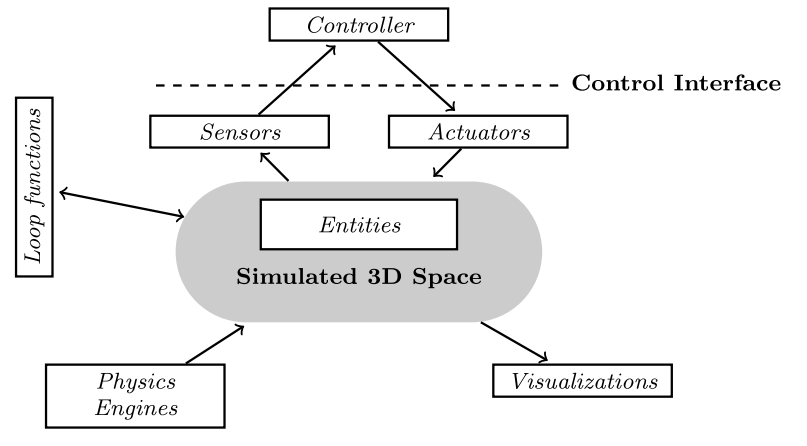
\includegraphics[scale=0.9]{figures/argos_architecture.png}
    \caption{Eine Übersicht über die Architektur von ARGoS. Übernommen aus \cite{Pinciroli2012}}
    \label{fig-argos-architecture}
  \end{figure}

  \subsection{Einführung in CollabSim}
    In CollabSim fungiert das Backend als zentrale Instanz für die Übertragung aller Daten und der Kommunikation. 
    Einerseits leitet es die bearbeiteten, für die Simulation erforderlichen Dateien zu einer virtuellen Maschine weiter und koordiniert die Ausführung der dort benötigten Befehle. 
    Andererseits sorgt es für die Echtzeitsynchronisation aller im Frontend entwickelten Dateien, um die Kollaboration zwischen allen Nutzern zu ermöglichen.

    Im Frontend wurde Angular als Entwicklungsframework eingeführt. 
    Angular wurde ausgewählt, weil es eine robuste Struktur für die Erstellung dynamischer und interaktiver Benutzeroberflächen bietet. 
    Es basiert auf TypeScript, einer Programmiersprache, die auf JavaScript aufbaut und zusätzliche Funktionen bietet, 
    um die Entwicklung robusterer Anwendungen zu unterstützen. 
    HTML (Hypertext Markup Language) wird verwendet, um die Struktur der Benutzeroberfläche zu definieren, 
    während CSS (Cascading Style Sheets) für das Design und das Aussehen der Anwendung zuständig ist. 
    Es erleichtert die Entwicklung durch eine modulare Architektur und bietet umfangreiche Bibliotheken und Tools, 
    die eine effiziente und skalierbare Entwicklung ermöglichen. 
    In den folgenden Abschnitten werde ich die einzelnen Komponenten von CollabSim vorstellen. 
    Einen Überblick über die gesamte Architektur bietet Abbildung \vref{fig-collabsim-architecture}.

    \begin{figure}[htpb]
      \centering
      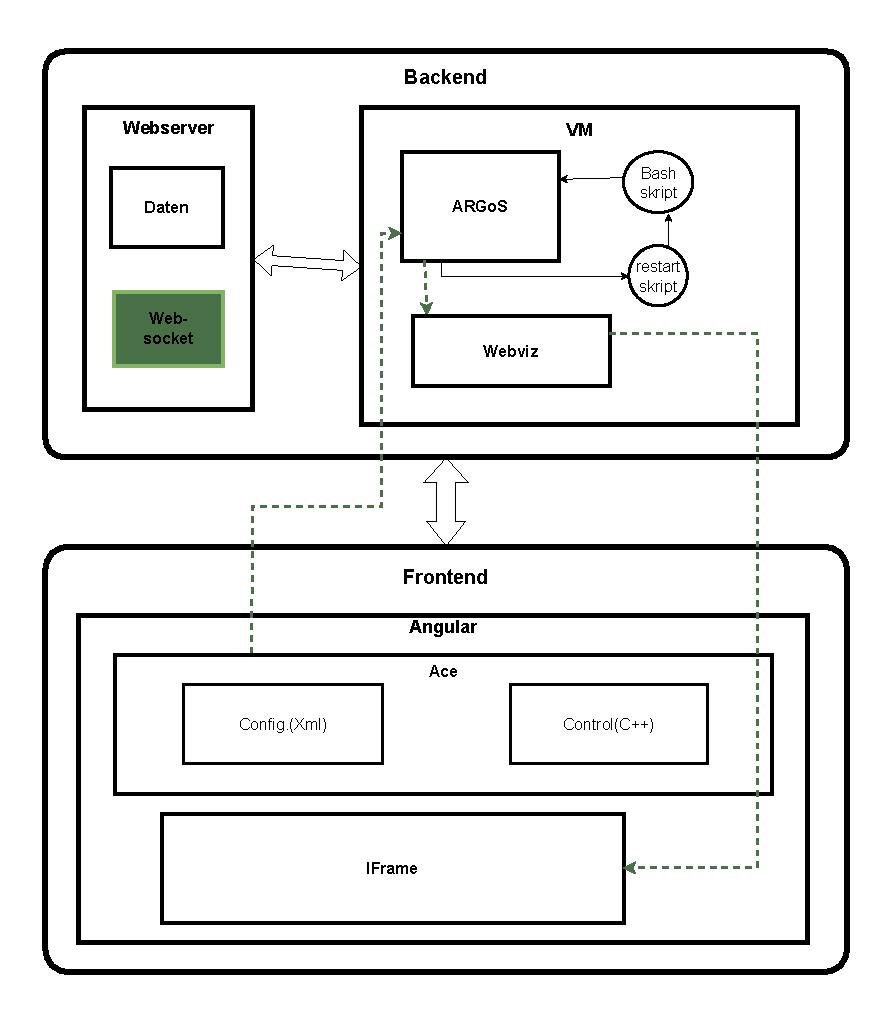
\includegraphics{figures/test8.drawio.pdf}
      \caption{Eine Übersicht über die Architektur von CollabSim}
      \label{fig-collabsim-architecture}
    \end{figure}



\section{Virtuelle Maschiene}
  Da ARGoS nur unter Linux und Mac OSX Betriebssystemen läuft, wird ein solches System für die Simulation benötigt. 
  Daher wurde zur Ausführung von ARGoS eine virtuelle Maschinne unter dem Ubuntu-Betriebssystem aufgesetzt.

  \subsection{ARGoS}
  ARGoS ist einer der wenigen Simulatoren, die Effizienz und Flexibilität in einem, für die Schwarmrobotik erforderlichem Maße umsetzen, 
  um die Echtzeitsimulation von Tausenden von Robotern zu ermöglichen\cite{Pinciroli2012}.
  Aufgrund seiner guten Performence ist er ein geeigneter Simulator im Bereich der Schwarmrobotik\cite{Shamshiri2018}. 
  In CollabSim wird ARGoS genutzt, um alle Aspekte der Simulation zu realisieren, einschließlich der Bewegungssteuerung der Roboter, 
  der Sensor- und Aktuator-Interaktionen sowie der Umgebungssimulation. 
  Diese umfassende Integration macht ARGoS zu einem Schlüsselelement für die Entwicklung und das Testen von Algorithmen in CollabSim.

  \subsection{Webviz}
  \label{webviz}
  Webviz ist ein für ARGoS entwickeltes Plugin\cite{ARGoS3-Webviz}, das die Visualisierung der simulierten Umgebung über den Browser ermöglicht. 
  Es hostet einen Websocket, der die verfügbaren Informationen von ARGoS nutzt und eine Anwendung erstellt, um die Simulation online darzustellen und zu steuern. 
  Dadurch können alle Benutzer, die die Website besuchen, dieselbe laufende Simulation sehen, was für die kollaborative Arbeit an dieser Simulation unerlässlich ist.

  \subsection{Zusätzliche Programme}
  Zusätzliche Programme innerhalb der virtuellen Maschiene, dienen der Synchronisation benötigter Daten und Koordination auszuführender Befehle, um die Aktuallität der Simulation zu gewährleisten.
  Hauptsächlich kommen ein auf Python basierender Webserver zum Einsatz, welcher ein Bash-Skript zur Aktualiesierung der Simulation aufruft.


\section{Webserver}
  Der Webserver, implementiert in Python, ist verantwortlich für die Verwaltung der gesamten Kommunikation 
  zwischen dem Frontend, Backend und der virtuellen Maschine.
  Der Server wird mit Hilfe der Python-Softwarepakete Flask und SocketIO bereitgestellt. 
  Flask ist ein leichtgewichtiges Webanwendungsframework, das für die schnelle Entwicklung von Webanwendungen entwickelt wurde und Werkzeuge, 
  Bibliotheken und Technologien zur Erstellung einer Webanwendung bereitstellt. 
  SocketIO ist eine Bibliothek, die Echtzeit-, bidirektionale und ereignisbasierte Kommunikation zwischen den Web-Clients und dem Server ermöglicht.

  Der Datenaustausch aller Komponenten ist durch einen Websocket verwirklicht, um eine möglichst schnelle Kommunikation zu bieten. 
  Im Webserver wurde der verwendetet Websocket mit SocketIO realisiert und unterstützt mehrere Ereignisse, 
  welche die Echtzeit-Synchronisation aller geschriebenen Texte gewährleisten.
  Andere Kommunikationsarten sind meist langsamer und damit für Echtzeitanwendungen weniger gut geeignet.
  Im Gegensatz ermöglichen Websockets eine ständige Verbindung, wodurch Daten kontinuierlich in beide Richtungen übertragen werden können.
  

\section{Ace}
  Der browserbasierte Code-Editor Ace \cite{ace} wird als Grundlage für alle Codebearbeitungen der Anwendung verwendet. 
  Ace ist ein vielseitiger Editor, der zahlreiche Funktionen bietet, darunter Syntax-Highlighting, automatische Einrückung und eine Such- und Ersetzungsfunktion. 
  Diese Eigenschaften machen Ace zu einem beliebten Werkzeug für Entwickler. Im Rahmen dieser Arbeit wird Ace in zwei Hauptanwendungsbereichen eingesetzt. 
  Zum einen wird die Konfigurationsdatei für ARGoS, geschrieben in XML, bearbeitet. Zum anderen wird der Kontrollalgorithmus, verfasst in C++, erstellt und modifiziert. 
  Diese beiden Instanzen verdeutlichen die Flexibilität und Leistungsfähigkeit von Ace bei der Bearbeitung von Code in verschiedenen Programmiersprachen und Anwendungsszenarien.

    \subsection{XML (Extensible Markup Language)} 
    Die XML-Datei ist für die Konfiguration der Szene verantwortlich. 
    In dieser Datei werden die verschiedenen Parameter und Einstellungen definiert, die für die Simulation in ARGoS notwendig sind. 
    Dazu gehören unter anderem die Spezifikation der Roboter, die Definition der Umgebung und die Initialisierung der Simulationselemente. 
    XML ist besonders geeignet für diese Aufgabe, da es eine strukturierte und leicht lesbare Art der Datenrepräsentation ermöglicht. 
    Durch die Verwendung von XML können Konfigurationsänderungen effizient vorgenommen und die Szenendefinitionen klar und verständlich dokumentiert werden.

    \subsection{C++}
    Eine zusätzliche Datei dient der Implementierung des Kontrollalgorithmus, 
    der von den vorhandenen Robotern genutzt wird und ist in der Programmiersprache C++ geschrieben. 
    C++ ist eine häufige Wahl für die Programmierung von Robotern, da sie eine hohe Ausführungsgeschwindigkeit und 
    präzise Speicherverwaltung bietet, die für Echtzeitanwendungen und komplexe Berechnungen unerlässlich sind.
    Besonders relevant wird dies, wenn das in der Simulation verwendete Programm auch auf den realen Roboter übertragen werden soll.
    Diese Datei enthält die Logik und Anweisungen, die es den Robotern ermöglichen, ihre Aufgaben autonom auszuführen. 
    Durch den Einsatz dieses Kontrollalgorithmus wird sichergestellt, dass die Roboter effizient und korrekt arbeiten, 
    indem sie auf verschiedene Umgebungsbedingungen und Anforderungen reagieren können. 
    Diese Datei spielt somit eine zentrale Rolle in der Steuerung und Koordination der robotischen Aktivitäten innerhalb des Simulationssystems.


\section{IFrame}
  Ein Iframe ist ein HTML-Element, das es ermöglicht, den Inhalt einer externen Webseite in eine andere Webseite einzubetten. 
  Dies macht es ideal, um die mit Webviz(siehe Abschnitt \ref{webviz}) erstellte Webanwendung in CollabSim zu integrieren. 
  Alternativ wäre die Entwicklung eines eigenen Clients möglich, um die Simulation darzustellen. 
  Diese Option erfordert jedoch erheblichen Zeitaufwand und bietet nur geringen Mehrwert für den Zweck dieser Arbeit.



%-----------------------------------user test---------------------------
\chapter{Nutzertest} 
\label{chapter-test}
%Wir wollen die Machbarkeit von solche Online SImulaiton tools vorstellen und auch abmessen wiefern sind wir vorangekommen.

  Die vorliegende Bachelorarbeit befasst sich mit der Entwicklung und Evaluierung eines kollaborativen Online-Simulationswerkzeugs für die Robotik. 
  Ziel der Arbeit ist es, die Machbarkeit und den Nutzen solcher Werkzeuge zu untersuchen und die Konkurenzfähigkeit gegenüber traditionellen Simulatoren in der Robotik, zu bewerten. 
  Dazu wird der entwickelte Simulator verwendet und von Teilnehmern einer Stichprobe hinsichtlich verschiedener Aspekte der Usability (Benutzerfreundlichkeit) bewertet.
  Dies soll auch dabei helfen einzuschätzen, inwiefern CollabSim einen erfolgreichen Prototypen des verfolgeten Ansatzes darstellt.
  In diesem Kapitel werden die Methoden der Untersuchung vorgestellt und diskutiert.


\section{Methodik}
  % daten + metriken
  In dieser Arbeit wurde zur Evaluierung des entwickelten Simulators CollabSim ein 
  Experiment mit freiwilligen Testpersonen aus der erwarteten Zielgruppe durchgeführt. 
  Anschließend wurde ein darauf aufbauender Fragebogen verwendet.

  Qualitative Daten basierend auf den, durch den Fragebogen erhaltende, Antworten wurden erfasst und analysiert.  
  Als Metriken zur Evaluierung des Simulationskonzepts wurden Zufriedenheit und Erlernbarkeit, Effizenz und Nützlichkeit sowie Konkurenzfähigkeit und Potenzial gewählt.
  Diese Metriken bieten Einblicke in die Nutzererfahrung und die Leistungsfähigkeit des Simulators. Sie reflektieren die subjektiven Einschätzungen der Teilnehmer.
  Zusätzlich wurden alle Durchläufe beobachtet, um besser nachzuvollziehen wo potenzielle Schhwierigkeiten auftreten.
  Dabei bestand kein Kontakt zu den Probanden, um diese nicht während der Durchführung zu beeinflussen.
  Bis auf die benötigte Zeit der einzelnen Durchgänge wurden keine weiteren quantitativen Daten aufgezeichnet. 
  In der anschließenden Bewertung wurden die gesammelten Ergebnisse statistisch analysiert.

  % - Erläuterung der Herangehensweise und Begründung der Methodenwahl \\
  Diese Entscheidung, für die Verwendung eines Fragebogens wurde aus mehreren Gründen getroffen.
  Erstens gibt es keine vorangegangenen Studien zu ähnlichen kollaborativen Online-Simulationswerkzeugen. 
  Daher wurde ein explorativer Ansatz gewählt, um umfassende erste Einblicke zu gewinnen.
  Zweitens war es schwierig eine große und diversifizierte Stichprobe zu rekrutieren. 
  Eine Herausforderung stellten der begrenzte Zeitrahmen sowie die Erreichbarkeit und Verfügbarkeit der recht spezifischen Zielgruppe von Studierenden, Absolventen und Forschenden im Bereich der Robotik dar.
  Ein Fragebogen stellte durch die Zeitbegrenzung eine praktikable und effiziente Methode dar, um die Forschungsfragen zu beantworten.
  Und trotz der begrenzten Teilnehmerzahl konnte durch diesen eine ausreichende Menge an Daten gesammelt werden, um erste Tendenzen zu beobachten.
  Zusätzlich bot diese Methode den Vorteil der Standardisierung durch Verwendung einer Skala und die Einfachheit bei der Datenerhebung und -auswertung. 
  Standardisierte Antworten ermöglichen eine leichte quantitative Auswertung und liefern vergleichbare Daten.
  Zusammenfassend lässt sich sagen, dass die Wahl der Methode durch verwandte Arbeiten und die spezifischen Rahmenbedingungen dieser Bachelorarbeit bestimmt wurde. 

  Der Fragebogen umfasst 15 Fragen, welche meist auf einer Skala von 1 (keien Zustimmunng) bis 10 (starke Zustimmung) bewertet werden.
  Die Fragen wurden zu großen Teilen aus den Werken von \cite{Schiller2023} und der System Usability Scale (SUS) \cite{Brooke1995} zur Bewertung der Usabillity übernommen und angepasst.
  Allerdings wurde nur ein Teil der, des System Usability Scale zugrundliegenden Fragen verwendet, da sich die Evaluation nicht nur auf die Usability von CollabSim beschränkt.
  Da keine einheitliche Evaluationsmethode für kollaborative online Simulatoren existiert, entstammen einige Fragen auch eher experimenteller Natur.
  Die Auswahl einer Teilmenge der SUS-Fragen, ergänzt durch spezifische zusätzliche Fragen, war eine methodische Entscheidung, 
  um eine präzisere und relevantere Bewertung im spezifischen Kontext dieser Studie zu ermöglichen. 
  Diese Vorgehensweise gewährleistet, dass die wichtigsten Aspekte der Usability erfasst werden und gleichzeitig Raum für die Untersuchung weiterer relevanter Themen bleibt.

\section{Experiment}
  % - Erläuterung des experimentellen Aufbaus und der Durchführung 
  % teilnehmer
  Das Experiment zur Evaluation des entwickelten Simulationswerkzeugs wurde mit 6 Teilnehmern, unter Verwenung des neu entwickelte Online-Simulationswerkzeuges, durchgeführt. 
  Die Teilnehmer waren Studierende und Absolventen der Robotik und verwandter Studiengänge, mit unterschiedlichen Vorkenntnissen in der Robotik.

  Ein Versuchsdurchlauf hat meist in etwa 20 Minuten in Anspruch genommen. Eine Zeitbeschränkung wurde nicht festgelegt. 
  Alle Probanden beantworteten identische Fragen und bearbeiteten die selben Aufgaben.
  In allen Durchläufen wurde die Zeit parallel gemessen und aufgezeichnet. Leider war es technisch nicht sichergestellt, 
  dass die Teilnehmer den gesamten Fragebogen ausfüllen mussten, um unvollständige Einreichungen zu vermeiden. 
  So kam es dazu, dass die Antwort auf eine Frage von einem Teilnehmer fehlt.
        
  % ablauf experiment
  Vor der Nutzung des Simulators ist es wichtig, die Qualität der Daten aus der Stichprobe zu analysieren. 
  Zu diesem Zweck durchliefen die Teilnehmer vor dem eigentlichen Experiment eine Vorab-Umfrage. 
  In dieser Umfrage wurden sie gebeten, ihre Fähigkeiten im Umgang mit den im Experiment verwendeten Technologien zu bewerten, 
  wie z.B. Computerkenntnisse, allgemeine Kenntnisse in der Robotik oder Erfahrungen in der Programmierung und Simulation von Robotersystemen.

  \begin{enumerate}
    \item 
    How many years of experience do you have in robotics?
    \item
    How often do you use computers? 
    \item
    How would you rate your knowlage about robotics? %/ = 32/6 = 5,..
    \item
    How would you rate your experience in programming robots or robot swarms? %/ 24/6 = 4  
    \item
    How would you rate your experience in simulating robots or robot swarms? %/ 25/6 = 4,..
    \end{enumerate}        
        
  Daraufhin folgte ein Experiment, in dem die Teilnehmer, unter der Verwendung von CollabSim, einfache Änderungen an einer vorgegebenen Simulationsumgebung vornehmen sollten.
  Diese Änderungen repräsentieren zwei typische Aufgaben bei der Simulation von Robotern. 
  Einerseits das Erstellen einer editierbaren Szene, in der ein Roboter zu Trainings- oder Testzwecken agiert.
  Andererseits das Testen, Anpassen oder Entwerfen von Kontrollalgorithmen zur Steuerung der verwendeten Roboter. 
  Die simulierte Umgebung ist in Abbildung \vref{fig-lösung} zu sehen.

  \begin{figure}[htpb]
    \centering
    \includegraphics{figures/Lösung xml.png}
    \caption{Die von den Teilnehmern in CollabSim bearbeitete Simulationsumgebung.}
    \label{fig-lösung}
  \end{figure}

  Nach der Nutzung des Simulationswerkzeugs sollten die Probanden die restlichen Fragen beantworten. 
  Diese zielten darauf ab, die Usability von CollabSim zu bewerten und eine Einschätzung des zu erforschenden Konzepts zu liefern.
  Die Teilnehmer bewerteten ihre Erfahrungen und die daraus resultierenden quantitativen Daten wurden anschließend statistisch ausgewertet, um aussagekräftige Ergebnisse zu erzielen.
  
  \begin{enumerate}
    \item 
    I would imagine that most people would learn to use this system very quickly. %= 45/6 = 7,.. median=8
    \item
    I needed to learn a lot of things before I could get going with this system. %= 18/6 = 3 median=3
    \item
    How do you rate the clarity and usability of the simulation? %= 47/6 = 7,.. median=8
    \item
    I found the various functions in this system were well integrated. %= 46/6 = 7,..  median=8.5
    \item
    I felt very confident using the tool. %= 45/6 = 7,..  median=8
    \item
    I  found the system very complicated to use. %= 16/6 = 2,. median=2.5
    \item
    I think that collaborative online simulation tools offer an advantage over traditional simulation tools. %= 47/5 = 8,.. median=10
    \item
    Compared to my previous experiences with similar tools, I made more progress using this simulation tool. %= 48/6 = 8   median=8
    \item
    I would recommend this simulation tool for similar tasks in the future. %= 49/6 = 8,.. median=8
    \item
    How would u rate the simulation tool? %= 46/6 = 7,.. median=8
    \end{enumerate}


  %Compared to my previous experiences with similar tools, I made more progress using this simulation tool. 
  % (in ease weil die meisten eher anfänger sind)
   % (in useabillity weil mehr progress) 
    % (in collab weil sim auch mit collab func funktionieren kann)
     % (in online weil die meisten zufriden waren mit online sim, wegen ease? einfach seite auf und los) 
      %    = 48/6 = 8   median=8

  Zusätzlich wurden weitere Fragen für den Versuchsdurchlauf mit zweier Paaren erstellt. 
  Diese Fragen sollten einen Vergleich, zwischen Einzelpersonnen und Gruppen, bei der Bearbeitung der Aufgaben ermöglichen.
  Außerdem ziehlten sie auf die Evaluation der integrierten kollaborativen Funktionen und ihr Zusammenspiel mit dem Gesamtsystem ab. 
  Sie waren nur zur Beantwortung vorgesehen, wenn das Experiment in einer Gruppe durchgeführt wurde. 
  Da nicht genügend Teilnehmer organisiert werden konnten, wurden keine Gruppen gebildet und diese Fragen damit hinfällig.
  Dementsprechend liegen keine Ergebnisse für diese Fragen vor und lassen Raum für weiterführende Untersuchungen.

\section{Hypothesentests}
  % kein t-test oder ähnliche Hypothesentest => deskriptive Statistiken
  Da ich nur eine Testgruppe habe und aufgrund der kleinen Stichprobengröße waren gängige Hypothesentests wie der T-Test oder der ANOVA-Test nicht anwendbar. 
  Stattdessen können deskriptive Statistiken verwendet werden, um die jeweiligen Mittelwerte und Standardabweichungen(SD) der Fragen zu analysieren und festzustellen, 
  ob die Teilnehmer den Simulator als benutzerfreundlich betrachten. Damit wird die Machbarkeit und der Nutzen des vorgestellten Ansatzes bewertet. 
  Es ist jedoch wichtig zu beachten, dass die Stichprobengröße nicht groß genug ist, um robuste Erkenntnisse aus der Interpretation dieser Ergebnisse zu gewinnen.
  Die Ergebnisse der Umfrage wird im folgenden Kapitel diskutiert.


  %quali
  %survey:
    
   %   post
    %    (teamwork)
     %   Wie wichtig war die Kommunikation und Koordination mit Ihrem Partner für den Erfolg der Aufgabe?
      %  Wie leicht war es, mit Ihrem Partner an der Simulation zusammenzuarbeiten?
       % Welche Aspekte der Simulation haben die Kollaboration unterstützt oder behindert?
        %Konnten Sie effektiv mit der Simulationsumgebung interagieren, um die gestellten Aufgaben zu lösen?
  %      Ich empfand die zussamenarbeit mit einem partner, bei der bearbeitung der  aufgaben, hilfreich
   %     Sie haben viel zeit investiert, um mit Ihrem Partner zu interagieren
%
 %       collab -- zusätzliche fragen
  %      2. I found the system/collab functions unnecessarily complex -> war collab unnötig
   %     9. I felt very confident using the system - usable/easy to understand, well integrated features
    %    10. I needed to learn a lot of things before I could get going with this system - no robo exp or not usable/understandable

      
  %quanti
   %       task completion  
    %      task completion time
          

\chapter{Ergebnisse und Diskussion}
\label{chapter-result}
%--Alternativen: Bezieht sich auf die Diskussion von alternativen Erklärungen oder Einschränkungen der Studie, um potenzielle Fehlerquellen zu identifizieren.
%--Validierung: Beschreibt die Überprüfung der Gültigkeit der Ergebnisse, sowohl intern als auch extern, und die Diskussion potenzieller Fehlerquellen oder Verzerrungen.
%--Interpretation: Umfasst die Diskussion und Interpretation der Ergebnisse, einschließlich möglicher Implikationen, Bedeutung und Relevanz für das Forschungsfeld.

In diesem Abschnitt werden die Ergebnisse der zuvor beschriebenen Nutzertests vorgestellt und anschließend diskutiert sowie interpretiert. 
Zudem werden die Forschungsfragen anhand der Ergebnisse diskutiert.

Die vorab gestellten Fragen der Umfrage dienten der Überprüfung der Eignung der Teilnehmer und ihrer Selbsteinschätzung bezüglich ihrer Kenntnisse in der Robotik. 
Sie stellen sicher, dass die Teilnehmer über ausreichendes Wissen und Erfahrung verfügen, um fundierte Rückmeldungen zur Simulationsumgebung zu geben.
Die Fragen nach der Durchführung des Experiments zielen darauf ab, die entwickelte Simulationsumgebung nach den Metriken Zufriedenheit und Erlernbarkeit, 
Effizienz und Nützlichkeit sowie Konkurenzfähigkeit und Potential zu bewerten.
Damit werden die wichtigsten Aspekte der Benutzerfreundlichkeit und die spezifischen Stärken und Schwächen der Simulationsumgebung erfasst und analysiert, 
was zu einer aussagekräftigen Beurteilung und möglichen Verbesserungsvorschlägen führt.




\section{Eignung und Selbsteinschätzung}
  Zu Beginn wurde nach der Anzahl der Jahre an Robotikerfahrung der Probanden gefragt. 
  Die zeitliche Erfahrung reichte dabei von 2 bis 5 oder mehr Jahren, wodurch ein breites Spektrum an Studierenden bis hin zu Masterabsolventen und 
  Berufseinsteigern abgedeckt wurde. 
  Es war wichtig, einen grundlegenden Wissens- und Erfahrungsstand vorauszusetzen, da für die sinnvolle und erfolgreiche Bearbeitung des Experiments grundlegende 
  Kenntnisse in Programmierung und Simulationen entscheidend sind.

  Tatsächlich lassen sich die sechs Teilnehmer basierend auf ihrer jahrelangen Erfahrung in zwei Dreiergruppen einteilen. 
  Die erste Gruppe besteht aus Studierenden mit 2 Jahren Erfahrung, die noch eher als Einsteiger angesehen werden können. 
  Die zweite Gruppe umfasst Teilnehmer mit über 2 Jahren Erfahrung in der Robotik und kann daher als fortgeschrittener betrachtet werden.
  In Abbildung \vref{fig-preq1} ist diese Aufteilung gut erkennbar. Auf die Auswirkungen dieser Gruppierung gehe ich im Abschnitt \ref{erfahrung} genauer ein.
  
  \begin{figure}[htpb]
    \centering
    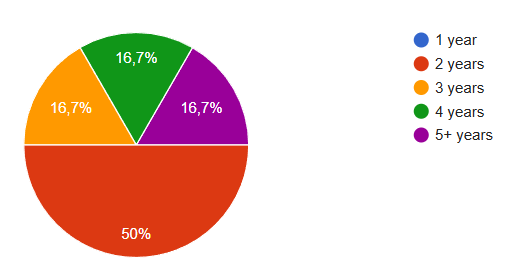
\includegraphics{figures/pre-question1.png}
    \caption{How many years of experience do you have in robotics? }
    \label{fig-preq1}
  \end{figure}


  Um die Vertrautheit der Probanden mit Computern einschätzen zu können, wurden sie nach ihrer täglichen Computernutzung befragt. 
  Es sollte sichergestellt werden, dass alle Teilnehmer über ausreichende Erfahrung mit Computern verfügen, um die gestellten Aufgaben erfolgreich bewältigen zu können. 
  Dies war insbesondere wichtig, da CollabSim als Onlinesimulator in modernen Browsern läuft und ein sicherer Umgang mit solchen Anwendungen erforderlich ist.
  Abbildung \vref{fig-preq2} zeigt, dass die Teilnehmer durchschnittlich mehrere Stunden pro Tag am Computer verbringen und somit ausreichend Erfahrung mitbringen sollten, 
  um den Simulator problemlos zu bedienen.
  
  \begin{figure}[htpb]
    \centering
    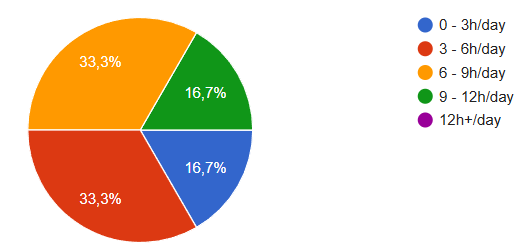
\includegraphics{figures/pre_question2.png}
    \caption{How often do you use computers? }
    \label{fig-preq2}
  \end{figure}

  Die drei restlichen, vorab gestellten Fragen dienten der Selbsteinschätzung. 
  Die Teilnehmer sollten ihre eigenen Kenntnisse in der Robotik sowie ihre Erfahrungen in der Programmierung und Simulation von Robotern oder Schwarmrobotern bewerten. 
  Diese Fragen wurden gestellt, um ein besseres Verständnis für den Hintergrund und das Erfahrungsniveau der Teilnehmer zu erhalten. 
  Dies ermöglicht eine differenziertere Analyse der Usability-Bewertung, indem die Ergebnisse in 
  Zusammenhang mit den Vorkenntnissen und Erfahrungen der Benutzer gesetzt werden können. 
  So werden eventuelle Unterschiede in der Wahrnehmung der Benutzerfreundlichkeit leichter identifiziert und besser interpretiert.
  Die Ergebnisse sind in den Abbildungen \vref{fig-preq3} - \vref{fig-preq5} dargestellt.
  
  \begin{figure}[htpb]
    \centering
    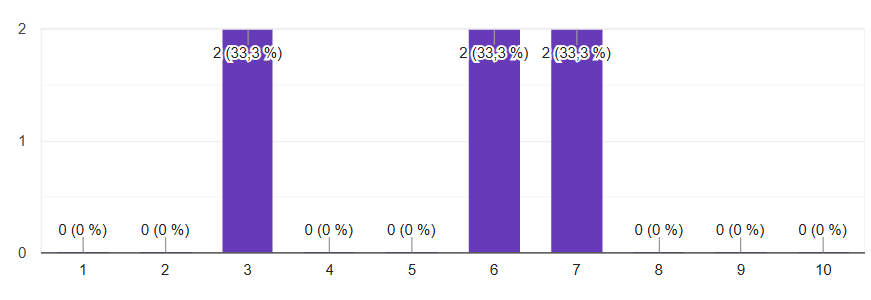
\includegraphics[scale=0.8]{figures/pre_question3.png}
    \caption{How would you rate your knowlage about robotics? 1-no knowlage, 10-expert}
    \label{fig-preq3}
  \end{figure}

  
  \begin{figure}[htpb]
    \centering
    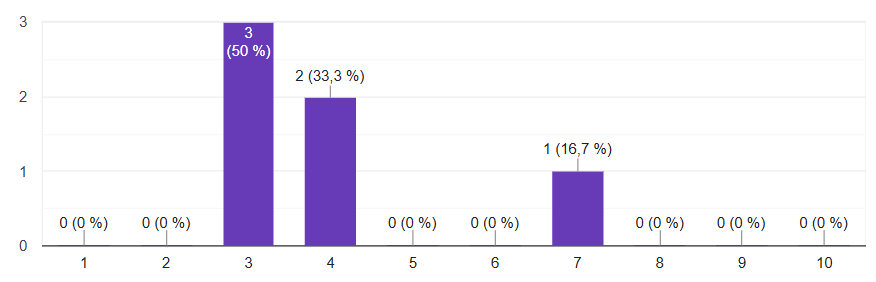
\includegraphics[scale=0.8]{figures/pre_question4.png}
    \caption{How would you rate your experience in programming robots or robot swarms? 1-no knowlage, 10-expert}
    \label{fig-preq4}
  \end{figure}


  \begin{figure}[htpb]
    \centering
    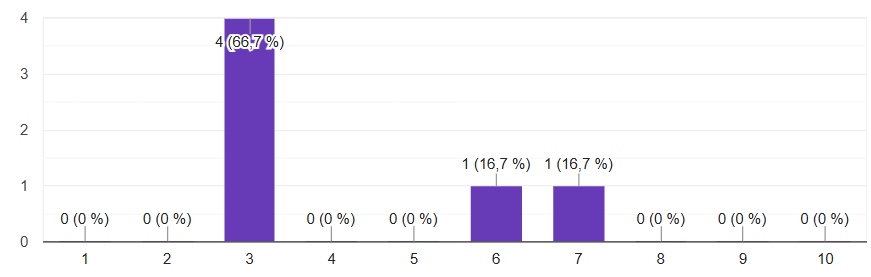
\includegraphics[scale=0.8]{figures/pre_question5.png}
    \caption{How would you rate your experience in simulating robots or robot swarms? 1-no knowlage, 10-expert}
    \label{fig-preq5}
  \end{figure}

  Es ist ein leichter, absehbarer Abstieg der bewerteten Kompetenz mit fallender Anzahl an Jahren im Bereich der Robotik erkennbar. 
  Ein klarer Zusammenhang zwischen der Selbsteinschätzung und anderen erhobenen Daten konnte jedoch nicht festgestellt werden. 
  Dies kann darauf hindeuten, dass die Selbsteinschätzung der Kompetenz möglicherweise zu stark von der subjektiven Wahrnehmung beeinflusst wird.

\section{Zufriedenheit und Erlernbarkeit}
  \begin{figure}[htpb]
    \centering
    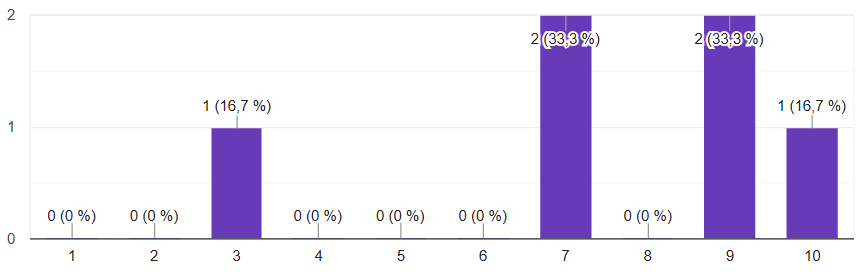
\includegraphics[scale=0.8]{figures/post_question1.png}
    \caption{I would imagine that most people would learn to use this system very quickly. 1-strongly disagree, 10-strongly agree}
    \label{fig-postq1}
  \end{figure}


  \begin{figure}[htpb]
    \centering
    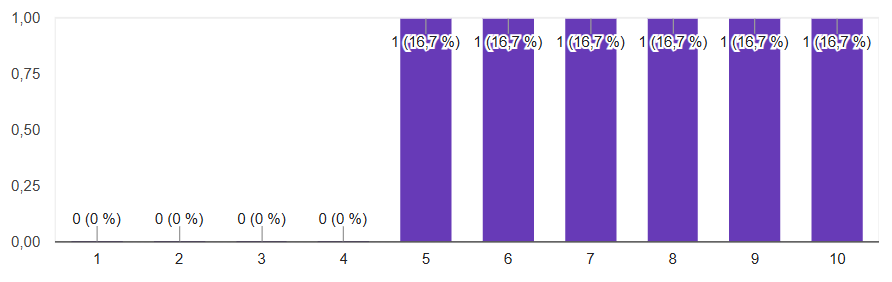
\includegraphics[scale=0.8]{figures/post_question5.png}
    \caption{I felt very confident using the tool. 1-strongly disagree, 10-strongly agree}
    \label{fig-postq5}
  \end{figure}

  \begin{figure}[htpb]
    \centering
    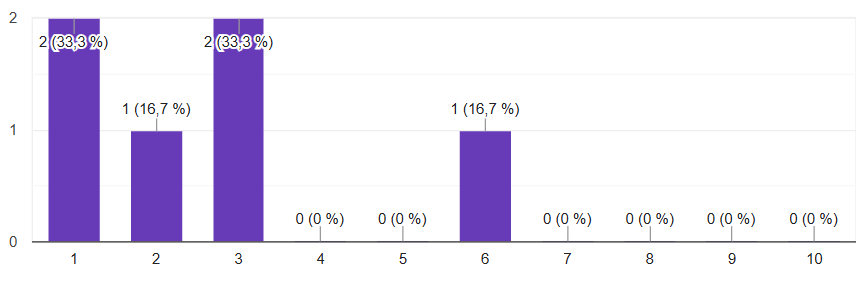
\includegraphics[scale=0.8]{figures/post_question6.png}
    \caption{I  found the system very complicated to use. 1-strongly disagree, 10-strongly agree }
    \label{fig-postq6}
  \end{figure}

  \begin{table}[htpb]
    \caption{Statistiken zur Zufriedenheit und Erlernbarkeit von CollabSim}
    \label{fig-ease}
    \centering
    \begin{tabular}{lp{1cm}l}
      \uzlhline
      \uzlemph{Aussage} & \uzlemph{Mittelwert} & \uzlemph{SD} \\ \uzlhline
      I would imagine that most people would learn to use this system very quickly. & 7.5 & 2.29 \\
      I felt very confident using the tool. & 7.5 & 1.71 \\ 
      I  found the system very complicated to use. & 2.67 & 1.7 \\ \uzlhline
    \end{tabular}
  \end{table}

  Die intuitive Nutzung einer Anwendung spielt eine entscheidende Rolle für die User Experience, die maßgeblich über den Erfolg eines Produkts entscheidet. 
  Um diesen Aspekt der Benutzerfreundlichkeit zu bewerten, wurden daher gezielte Fragen in den Fragebogen aufgenommen. 
  Diese Fragen zielen darauf ab, zu erfassen, wie gut die Anwendung von den Nutzern verstanden und effektiv genutzt wird. 


  

  Abbildungen \vref{fig-postq1} - \vref{fig-postq6} und die Auswertung in Tabelle \ref{fig-ease} zeigen, dass sich die Teilnehmer recht selbstbewusst und sicher bei der Nutzung von CollabSim fühlten.
  Die Ergebnisse zeigen, dass die Benutzer mit der Anwendung zufrieden waren und sich kompetent im Umgang mit den Funktionen fühlten.



\section{Effizenz und Nützlichkeit}
  \begin{figure}[htpb]
    \centering
    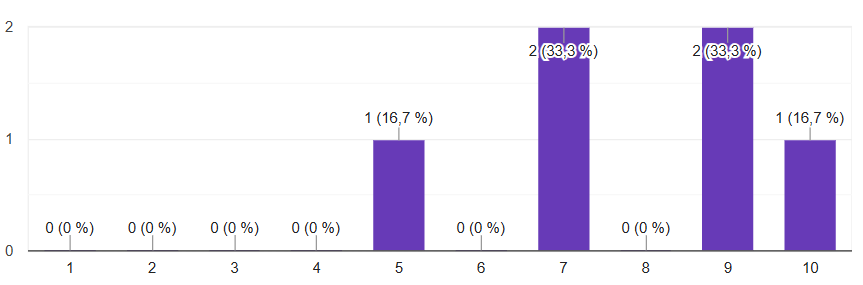
\includegraphics[scale=0.8]{figures/post_question3.png}
    \caption{How do you rate the clarity and usability of the simulation? 1-not usable, 10-very usable }
    \label{fig-postq3}
  \end{figure}

  \begin{figure}[htpb]
    \centering
    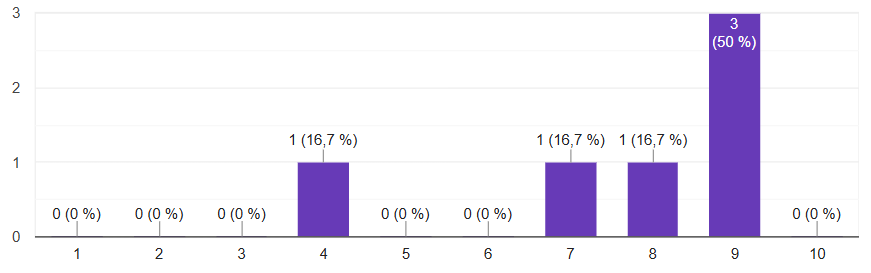
\includegraphics[scale=0.8]{figures/post_question4.png}
    \caption{I found the various functions in this system were well integrated. 1-strongly disagree, 10-strongly agree }
    \label{fig-postq4}
  \end{figure}


  \begin{table}[htpb]
    \caption{Statistiken zur Effizenz und Nützlichkeit von CollabSim}
    \label{fig-effi}
    \centering
    \begin{tabular}{lp{1cm}l}
      \uzlhline
      \uzlemph{Aussage} & \uzlemph{Mittelwert} & \uzlemph{SD} \\ \uzlhline
      How do you rate the clarity and usability of the simulation? & 7.83 & 1.68 \\
      I found the various functions in this system were well integrated. & 7.67 & 1.8 \\ \uzlhline
    \end{tabular}
  \end{table}

  Natürlich sollte man mit einer Anwendung auch effizient arbeiten können. 
  Dementsprechend ist es wichtig, dass die Funktionen klar, einfach verständlich und nutzbar sind. 
  Auch hier konnte CollabSim überzeugen. 
  Die zugehörigen Fragen sind in den Abbildungen \vref{fig-postq3} und \vref{fig-postq4} aufgelistet. 
  Die Wertungen der Fragen in Tabelle \ref{fig-effi} deuten darauf hin, dass die Teilnehmer der Meinung waren, 
  die Funktionen seien gut integriert und das System insgesamt nützlich. 
  Die Ergebnisse bestätigen, dass CollabSim eine solide Grundlage für eine effiziente Arbeitsumgebung bietet.




\section{Konkurenzfähigkeit und Potential}
  Es lässt sich sagen, dass dieses Online-Simulationswerkzeug insgesamt gut von den Nutzern bewertet wurde, was in den Abbildungen \vref{fig-postq8} - \vref{fig-postq10} ersichtlich ist. 
  Auch im Vergleich zu traditionellen Simulatoren scheint es besser abzuschneiden.

  Die Probanden waren der Meinung, dass kollaborative Online-Simulatoren große Vorteile gegenüber herkömmlichen Simulatoren bieten können. 
  Obwohl dies nur ihre Einschätzung widerspiegelt, ist ein so deutliches Ergebnis dennoch aussagekräftig (siehe Abbildung \vref{fig-postq7}). 
  Der potenzielle Nutzen wurde intuitiv erkannt und scheint gerechtfertigt, wenn man die Vorteile und die steigende Nachfrage nach kollaborationsfähigen Werkzeugen in vielen Bereichen betrachtet.
  Das Feedback zeigt, dass die kollaborativen Funktionen als besonders vorteilhaft angesehen wurden, 
  was darauf hinweist, dass solche Werkzeuge das Potenzial haben, die Effizienz und Produktivität in teamorientierten Arbeitsumgebungen signifikant zu erhöhen. 
  Dies unterstreicht die Relevanz und den Mehrwert von kollaborativen Online-Simulatoren in der modernen, vernetzten Arbeitswelt.

  \begin{figure}[htpb]
    \centering
    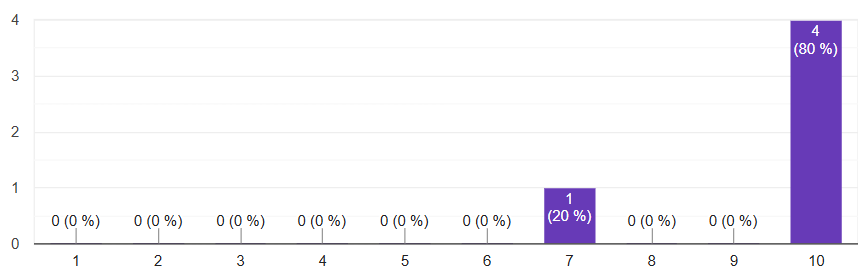
\includegraphics[scale=0.8]{figures/post_question7.png}
    \caption{I think that collaborative online simulation tools offer an advantage over traditional simulation tools. 1-strongly disagree, 10-strongly agree }
    \label{fig-postq7}
  \end{figure}
  
  \begin{figure}[htpb]
    \centering
    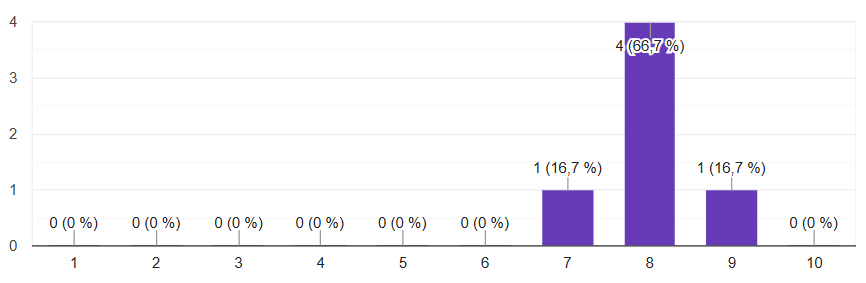
\includegraphics[scale=0.8]{figures/post_question8.png}
    \caption{Compared to my previous experiences with similar tools, I made more progress using this simulation tool. 1-strongly disagree, 10-strongly agree }
    \label{fig-postq8}
  \end{figure}
  
  Im Gegensatz zu anderen Simulationen empfanden die Probanden eine deutliche Effizenzsteigerung duch den Einsatz von CollabSim, wie in Abbildung \vref{fig-postq8} und anhand der niedrigen Standardabweichungen (siehe Tabelle \ref{fig-pot}), zu sehen ist.
  Gerade für Anfänger ist die korrekte Einrichtung vieler Simulatoren meist kompliziert und zeitintensiv, wohingegen CollabSim in jedem modernen Browser aufrufbar ist.  
  Dadurch kann diese Zeit eingespart werden, wesshlab das Konzept eines webbasierten Simulators vermutlich wesentlich einfacher, schneller und effizienter wirkt.  

  \begin{figure}[htpb]
    \centering
    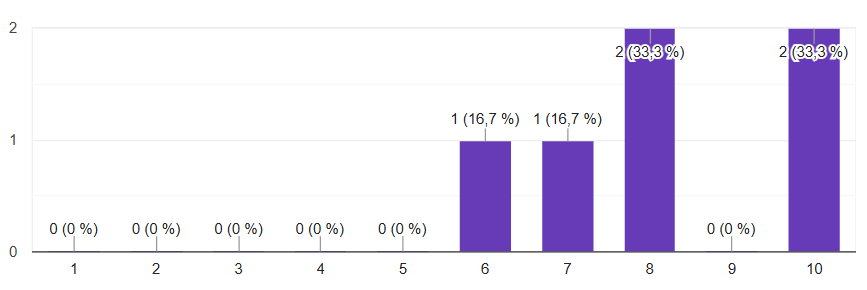
\includegraphics[scale=0.8]{figures/post_question9.png}
    \caption{I would recommend this simulation tool for similar tasks in the future. 1-strongly disagree, 10-strongly agree }
    \label{fig-postq9}
  \end{figure}
  
  \begin{figure}[htpb]
    \centering
    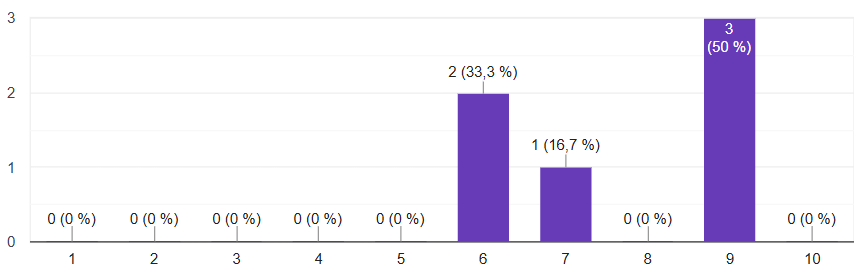
\includegraphics[scale=0.8]{figures/post_question10.png}
    \caption{How would u rate the simulation tool? 1-very bad, 10-very good }
    \label{fig-postq10}
  \end{figure}
  
  \begin{table}[htpb]
    \caption{Statistiken zur Konkurenzfähigkeit und Potential von CollabSim}
    \label{fig-pot}
    \centering
    \begin{tabular}{lp{1cm}l}
      \uzlhline
      \uzlemph{Aussage} & \uzlemph{Mittelwert} & \uzlemph{SD} \\ \uzlhline
      I think that collaborative online simulation tools offer \\an advantage over traditional simulation tools. & 9.4 & 1.2 \\\uzlhline
      Compared to my previous experiences with similar tools, \\I made more progress using this simulation tool. & 8 & 0.57 \\\uzlhline
      I would recommend this simulation tool for similar tasks in the future. & 8.17 & 1.46 \\\uzlhline
      How would u rate the simulation tool? & 7.67 & 1.38 \\ \uzlhline
    \end{tabular}
  \end{table}
  
  Das Konzept und der Simulator selbst, scheinen auch überzeugt zu haben. 
  Dies spiegelt sich in der Bewertung von CollabSim mit durchschnittlich 7,67 Punkten wieder. 
  Die Ergebnisse werden in Abbildung \vref{fig-postq10} aufgezeigt.
  Die statistischen Kennzahlen zu den Antworten werden in Tabelle \ref{fig-pot} angezeigt.


\section{Erfahrung}
\label{erfahrung}
  Die Erfahrung der einzelnen Teilnehmer erwies sich als wesentlicher Faktor für die Bewertung des Simulators. 
  Bei vielen Fragen wurde der Simulator von den unerfahrenen Nutzern leicht bis deutlich schlechter bewertet als von den erfahreneren Teilnehmern. 
  Teilt man die Probanden in eine Gruppe von Anfängern, mit bis zu 2 Jahren Erfahrung, und eine Gruppe von Fortgeschrittenen, mit über 2 Jahren Erfahrung in der Robotik, wird diese Tendenz deutlich.

  Beispielsweise bei der Frage, ob der Proband der Meinung sei, dass er für eine effiziente Nutzung noch viel lernen müsse, ist ein großer Unterschied feststellbar. 
  In Abbildung \vref{fig-postq2} und in Tabelle \ref{fig-exp} sind die entsprechenden Antworten und Statistiken.
  Die Anfänger lagen mit einer durchschnittlichen Wertung von 4 doppelt so hoch wie die fortgeschrittene Gruppe.
  Also hatten sie den Eindruck, dass sie noch einiges dazu lernen müssten.

  \begin{figure}[htpb]
    \centering
    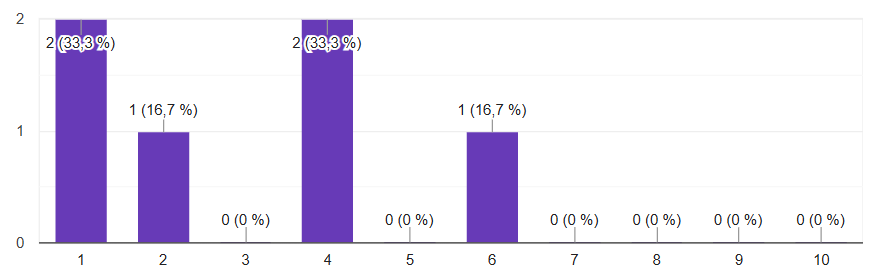
\includegraphics[scale=0.8]{figures/post_question2.png}
    \caption{I needed to learn a lot of things before I could get going with this system. 1-strongly disagree, 10-strongly agree }
    \label{fig-postq2}
  \end{figure}

  \begin{table}[htpb]
    \caption{Statistiken zur Erfahrung der Probanden}
    \label{fig-exp}
    \centering
    \begin{tabular}{lp{1cm}l}
      \uzlhline
      \uzlemph{Aussage} & \uzlemph{Mittelwert} & \uzlemph{SD} \\ \uzlhline
      I needed to learn a lot of things before I could get going with this system. & 3 & 1.82 \\ \uzlhline
    \end{tabular}
  \end{table}

  In diesem Fall scheint der Unterschied aufgrund der geringeren Erfahrung absehbar, jedoch beeinflusst dieser Trend die Wertung auch in anderen Bereichen. 
  Die unerfahrenere Gruppe bewertet auch die Fragen zum schnellen Erlernen des Systems, zur Integration der Funktionen und zum Selbstbewusstsein bei der Nutzung deutlich schlechter. 
  Auch eine leicht geringere Gesamtwertung und Empfehlung scheinen die Folge zu sein. 
  In den Abbildungen \vref{fig-group1} - \vref{fig-group6} wurden zur Veranschaulichung die Antworten einiger Fragen nach den Gruppen aufgeteilt.

  \begin{figure}[htpb]
    \centering
    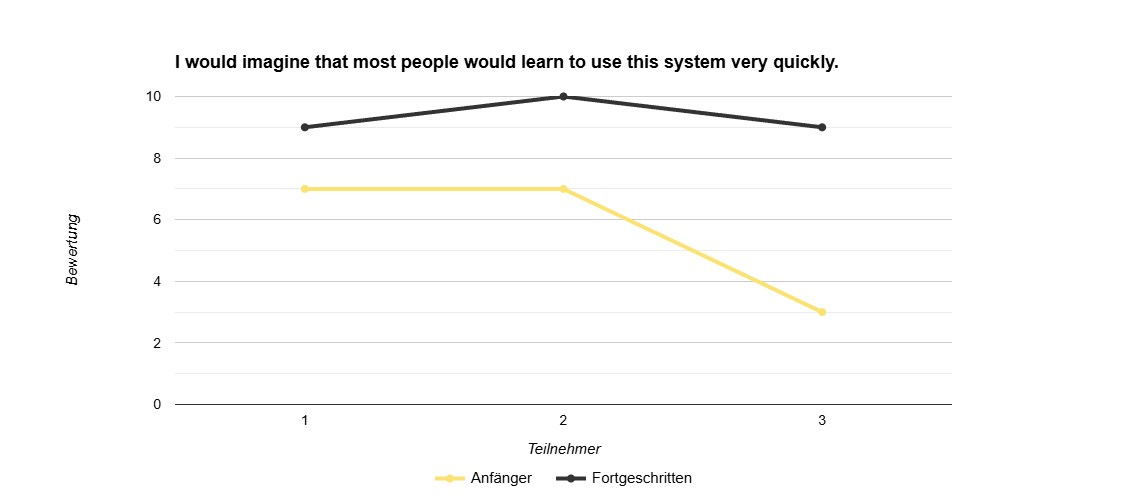
\includegraphics[scale=0.4]{figures/group1.png}
    \caption{Vergleich der Bewertungen der Aussage ``I would imagine that most people would learn to use this system very quickly.'' zwischen den Teilnehmern mit unterschiedlicher Erfahrung. 
              Jeder Punkt in der Abbildung repräsentiert einen Teilnehmer. Gelbe Punkte stehen für unerfahrenere Teilnehmer, schwarze Punkte für erfahrene Teilnehmer. }
    \label{fig-group1}
  \end{figure}

  \begin{figure}[htpb]
    \centering
    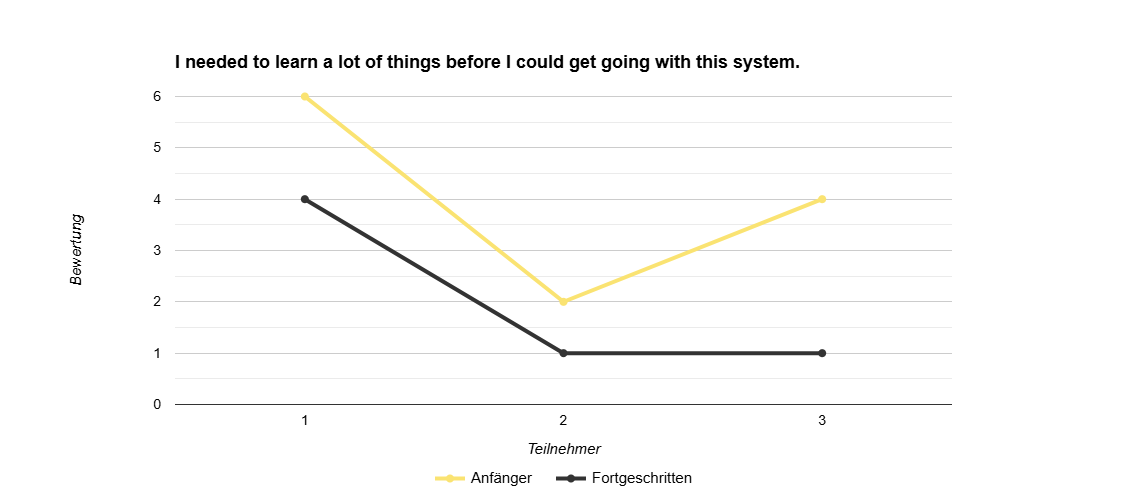
\includegraphics[scale=0.4]{figures/group2.png}
    \caption{Vergleich der Bewertungen der Aussage ``I needed to learn a lot of things before I could get going with this system.'' zwischen den Teilnehmern mit unterschiedlicher Erfahrung. 
    Jeder Punkt in der Abbildung repräsentiert einen Teilnehmer. Gelbe Punkte stehen für unerfahrenere Teilnehmer, schwarze Punkte für erfahrene Teilnehmer. }
    \label{fig-group2}
  \end{figure}

  \begin{figure}[htpb]
    \centering
    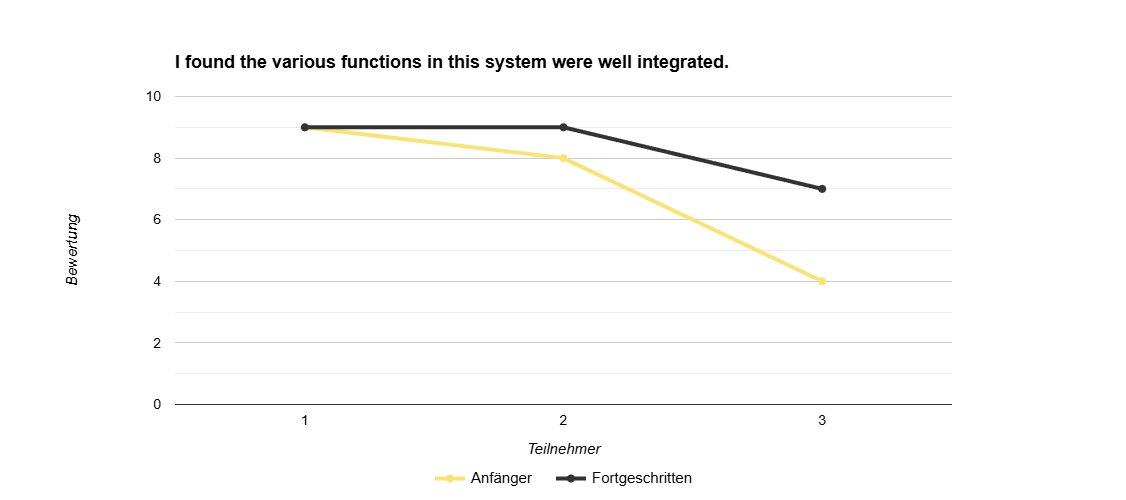
\includegraphics[scale=0.4]{figures/group3.png}
    \caption{Vergleich der Bewertungen der Aussage ``I found the various functions in this system were well integrated.'' zwischen den Teilnehmern mit unterschiedlicher Erfahrung. 
              Jeder Punkt in der Abbildung repräsentiert einen Teilnehmer. Gelbe Punkte stehen für unerfahrenere Teilnehmer, schwarze Punkte für erfahrene Teilnehmer. }
    \label{fig-group3}
  \end{figure}

  \begin{figure}[htpb]
    \centering
    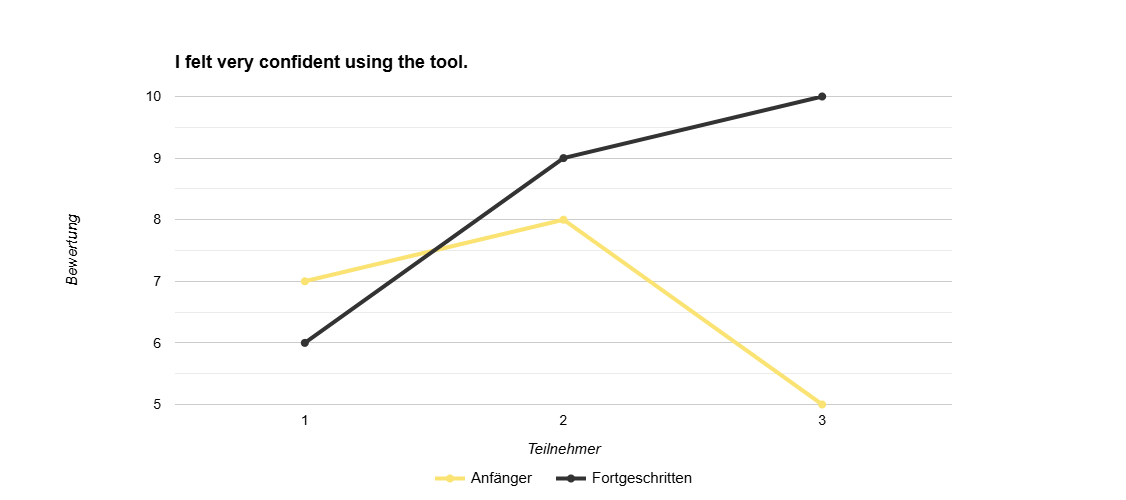
\includegraphics[scale=0.4]{figures/group4.png}
    \caption{Vergleich der Bewertungen der Aussage ``I felt very confident using the tool.'' zwischen den Teilnehmern mit unterschiedlicher Erfahrung. 
              Jeder Punkt in der Abbildung repräsentiert einen Teilnehmer. Gelbe Punkte stehen für unerfahrenere Teilnehmer, schwarze Punkte für erfahrene Teilnehmer. }
    \label{fig-group4}
  \end{figure}

  \begin{figure}[htpb]
    \centering
    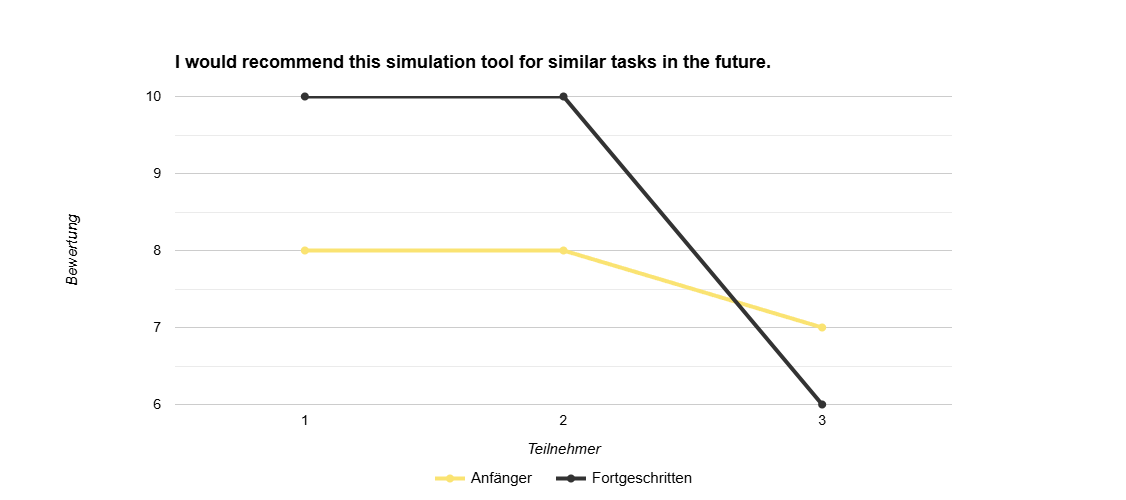
\includegraphics[scale=0.4]{figures/group5.png}
    \caption{Vergleich der Bewertungen der Aussage ``I would recommend this simulation tool for similar tasks in the future.'' zwischen den Teilnehmern mit unterschiedlicher Erfahrung. 
              Jeder Punkt in der Abbildung repräsentiert einen Teilnehmer. Gelbe Punkte stehen für unerfahrenere Teilnehmer, schwarze Punkte für erfahrene Teilnehmer. }
    \label{fig-group5}
  \end{figure}

  \begin{figure}[htpb]
    \centering
    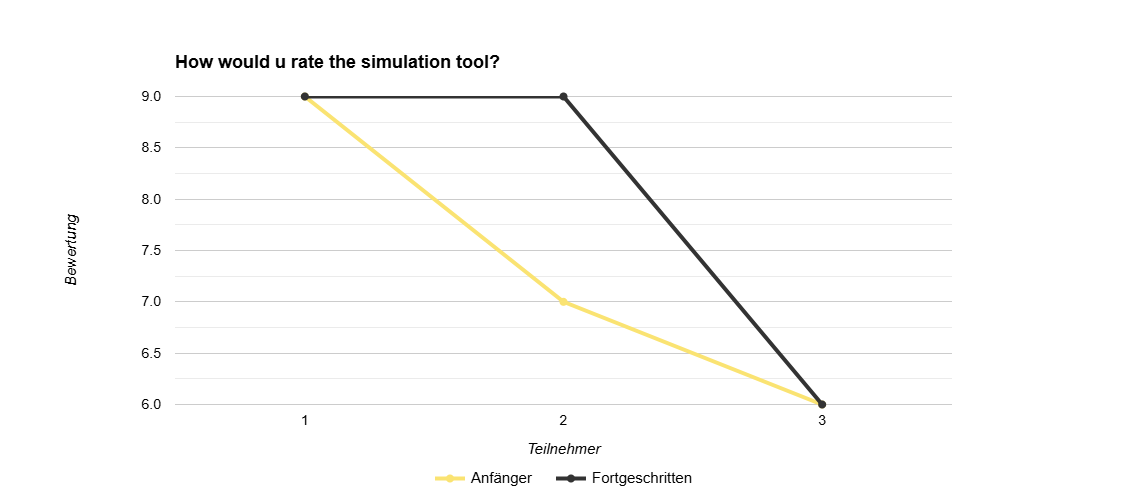
\includegraphics[scale=0.4]{figures/group6.png}
    \caption{Vergleich der Bewertungen der Aussage ``How would u rate the simulation tool?'' zwischen den Teilnehmern mit unterschiedlicher Erfahrung. 
              Jeder Punkt in der Abbildung repräsentiert einen Teilnehmer. Gelbe Punkte stehen für unerfahrenere Teilnehmer, schwarze Punkte für erfahrene Teilnehmer. }
    \label{fig-group6}
  \end{figure}

  Diese Unterschiede in den Bewertungen unterstreichen die Bedeutung von ausreichend Erfahrung und Wissen, um die Simulation sinnvoll nutzen zu können. 
  Sie bieten zudem wertvolle Einblicke für mögliche Optimierungen und Anpassungen des Systems an die Bedürfnisse verschiedener Benutzergruppen.





\section{Limitationen und Fehlermöglichkeiten}
  Leider konnte mit dem durchgeführten Experiment kein direkter Vergleich zwischen der Verwendung herkömmlicher Simulatoren und der kollaborativen Nutzung mit CollabSim durchgeführt werden. 
  Da die Versuchsgruppe sehr klein ausfiel, liefern die Ergebnisse eher Indizien und Tendenzen als klare Evidenz. 
  Zudem ist der Hintergrund für die Bewertung der Fragen nicht vollständig klar und nachvollziehbar, was Raum für Spekulationen lässt. 
  Weitere Studien mit größeren und diversifizierteren Teilnehmergruppen wären wünschenswert, um die Validität und Aussagekraft der Ergebnisse weiter zu stärken.

\section{Schlussfolgerungen}
  %- Interpretation der Ergebnisse im Hinblick auf deine Forschungsfrage(n) und Hypothesen
  %- Interpretation deiner Ergebnisse im Kontext der vorhandenen Literatur 
  %- Reflexion über mögliche Einschränkungen deiner Studie / Reflexion über die Stärken und Schwächen der durchgeführten Studie und mögliche Verbesserungen
  %- Diskussion über die praktischen Implikationen der Ergebnisse für die Schwarmrobotik-Forschung und -Entwicklung


  
  %online
   %     ease => online easier
    %    useabillity gut => online funktioniert

 
  Die vorhandenen Ergebnisse erlauben keine eindeutigen Schlussfolgerungen hinsichtlich des kollaborativen Aspekts des Simulators. 
  Dennoch lässt sich festhalten, dass es keinen Hinweis darauf gibt, dass die dafür notwendigen Funktionen zu Einschränkungen in der Usability für Einzelnutzer führen würden. 
  Das sehr eindeutige Ergebnis bei der Bewertung des Potenzials kollaborativer Simulatoren deutet ebenfalls auf mögliche Vorteile gemeinsamer Nutzung und die Bereitschaft der Zielgruppe hin, dieses Konzept zu akzeptieren.

  Die recht klaren Ergebnisse bezüglich der Benutzerfreundlichkeit von CollabSim lassen den Schluss zu, dass die Einfachheit der Nutzung eines Online-Simulators einen klaren 
  Vorteil gegenüber Offline-Simulatoren bietet und den Umgang mit Simulatoren vereinfacht. 
  Die positiv bewerteten Metriken zeigt zudem, dass der Ansatz eines Online-Simulators keine Einbußen in der Usability nach sich zieht, sondern im Gegenteil zu einer Steigerung der Effizienz führt. 
  Dies stützt die Folgerung, dass Benutzer von der einfacheren Handhabung profitieren und die Effizienz ihrer Arbeitsprozesse steigern können.

  Interpretiert man die Auswertung im Kontext der Forschungsfrage, ergibt sich die Tendenz, dass CollabSim erfolgreich die Herausforderungen der Usabillity meistert und dabei die Effizienz der Nutzung erhöht.
  Besonders bei Nutzern mit genügend Erfahrung kann CollabSim überzeugen. 
  Damit ist es ein erfolgreicher Prototyp und zeigt die Machbarkeit und gibt Einblicke in die Vorteile des vorgestellten Konzepts.
  Es bleibt jedoch unklar, ob der kollaborative online Ansatz für alle Arten von Simulatoren in der Robotik gleichermaßen sinnvoll ist.




      

\chapter{Zusammenfassung und Ausblick}
\label{chapter-con}
%(5-10/100, 2-3 Seiten)

Zum Abschluss dieser Arbeit werden die wichtigsten Erkenntnisse und daraus resultierenden Schlussfolgerungen aufgezeigt. 
Außerdem werde ich auf potenzielle Anwendungen von kollaborativem Arbeiten in der Schwarmrobotik eingehen und 
die Bedeutung der Forschungsergebnisse für die Robotik und Simulation bewerten.

  Die Erkenntnisse aus der Untersuchung von CollabSim bieten wertvolle Einblicke. 
  Die Studie zeigt, dass der Online-Simulator gegenüber traditionellen, offline basierten Simulatoren klare Vorteile bietet. 
  Insbesondere wurde die erfolgreiche Umsetzung wichtiger Aspekte der Usability und das große Potenzial des Simulationskonzepts durch die Teilnehmer bestätigt. 
  Erfahrene Nutzer bewerteten CollabSim tendenziell positiver, was die Relevanz entsprechender Kenntnisse unterstreicht. 
  Diese Ergebnisse legen nahe, dass kollaborative Online-Simulatoren wie CollabSim nicht nur die Benutzerzufriedenheit steigern können, 
  sondern auch die Effizienz in der Robotikentwicklung fördern könnten, indem sie komplexe Arbeitsprozesse vereinfachen und die Zusammenarbeit verbessern.

    Weitere Untersuchungen bezüglich der kollaborativen Aspekte von CollabSim wären für eine fundierte Einschätzung notwendig. 
    Hierfür war der Nutzertest mit einer zusätzlichen Testgruppe, welche den Simulator gemeinsam in Zweiergruppen bedient, geplant. 
    Dies scheiterte jedoch an einem Mangel an Zeit und Probanden.
    Zusätzliche Daten zur Erfassung der Leistungen der Probanden und ihrer Zusammenarbeit wären hier entscheidend. 
    Beispielsweise könnte überprüft werden, inwieweit die Aufgaben unter den Gruppenmitgliedern aufgeteilt wurden. 
    Auch die Häufigkeit und die aufgewendete Zeit für die Kommunikation könnten gemessen werden, um mögliche Zusammenhänge zu untersuchen. 
    Durch größere Stichproben könnte die Evidenz der Studienergebnisse weiter gestärkt werden.
    
    Die unerforschte Natur von kollaborativen, webbasierten Robotiksimulatoren lässt viel Raum für weiterführende Arbeiten. 
    Weitere Untersuchungen, worin genau die Vorteile solcher Werkzeuge liegen, könnten zum Besseren Verständniss dieser beitragen.
    Ebenso ist noch Unklar in welchen spezifischen Bereichen diese Vorteile besonders zur Geltung kommen könnten.

    Eine Zukunft, in der Simulationen in der Robotik kollaborativ in Onlinesimulatoren durchgeführt werden, könnte anhand der Ergebnisse als eine mögliche Konsequenz betrachtet werden. 
    Diese Entwicklung hat das Potenzial, die Hardware- und Softwareentwicklung in der Robotik grundlegend zu verändern.
    



          
        
  


 








   
   





% Normally, the bibliography comes next at this point. Do *not* (try
% to) include further indices and tables like an index or
% a list of figures or a list of tables or such things. Nobody
% actually uses them and they just use up space. 
%
% You *can* however include a glossary, if this seems appropriate. It
% goes here as an unnumbered chapter. Most thesis will *not* need a
% glossary: a well-written text (re)explains strange words and
% concepts as necessary. However, there are situations where a
% glossary may be helpful.








%%%
% 
% Bibliographies
%
%%%
%
% The uzl-thesis class will load biblatex for the bibliography
% management. This is a powerful package, see its documentation for
% details. The styles will be setup correctly and automatically by
% choosing one of the two style keys as described earlier.
%
% In order for the bibliography to work, run latex in the following
% order (which is the standard order):
% 
% > lualatex thesis-example
% > bibtex thesis-example
% > lualatex thesis-example
% 
% Add BibTeX files using \addbibresource or use the {bibtex entries}
% environment (see below).
%
%%%
%
% Although everyting is normally setup automatically, you can change
% the options passed to biblatex using the key 'biblatex';
% for instance,
%
%   \UzLThesisSetup{biblatex={firstinits=false}}
%
% will switch off shortened first names. Normally, you will not need
% this key in your preamble. 
% 
% Note that the bibtex program is used as the 'backend' of biblatex
% by default (rather than biber, which is the preferred program of
% biblatex). This means that you can (and must) run *bibtex* after you
% have run lualatex on your thesis. If you wish to use biber instead
% of bibtex, say 'biblatex={backend=biber}'. 
% 
%%%
%
% The following environment is optional. It allows you to keep the
% bibtex entries for your thesis right here in the thesis file. What
% happens is that each time this tex file is processed, the contents
% of the following environment gets written to the file
% \jobname-bibtex-entries.bib (this file gets overwritten each
% time). Independently, \addbibresource{\jobname-bibtex-entries.bib}
% is always called if the file \jobname-bibtex-entries.bib
% exists. 
%
% In result, you can edit and keep the bibliography's bibtex entries
% right here. If you change something here, run latex, then bibtex,
% then latex once more.
%
% If you would like to manage the bibtex entries in a separate file,
% remove the below environment, delete the \jobname-bibtex-entries.bib
% file and instead write
%
% \addbibresource{filename-of-your-bibtex-file.bib}
%
% in the preamble.
%
%%%


% !!!!!!!!!!!!!!!!!!!!!!!!!!!!!!!!!!
% !!! Your action is needed here !!!
% !!!!!!!!!!!!!!!!!!!!!!!!!!!!!!!!!!
%
% Replace following example entries with the ones of your thesis.

\begin{bibtex-entries}
% 2
@Book{Haber2012,
  author =       {Adam Haber, Matthew McGill, Claude Sammut},
  title =        {jmeSim: An Open Source, Multi Platform Robotics Simulator},
  institution =    {School of Computer Science and Engineering, UNSW},
  year =         {2012},
}
% 3
@Book{Shamshiri2018,
  author =       {Redmond Ramin Shamshiri},
  title =        {Simulation software and virtual environments for acceleration of 
                  agricultural robotics: Features highlights and performance comparison},
  institution =    {University of Illinois at Urbana Champaign},
  year =         {2018},
}
% 5
@Book{Pinciroli2012,
  author =       {Carlo Pinciroli, Vito Trianni, Rehan O’Grady, Giovanni Pini, Arne Brutschy,
                  Manuele Brambilla, Nithin Mathews, Eliseo Ferrante, Gianni Di Caro,
                  Frederick Ducatelle, Mauro Birattari, Luca Maria Gambardella, Marco Dorigo},
  title =        {ARGoS: a modular, parallel, multi-engine simulator for multi-robot systems},
  publisher =    {Springer Science+Business Media New York 2012},
  year =         {2012},
  doi =          {10.1007/s11721-012-0072-5},
}
% 6
@Book{Castillo2010,
  author =       {Patricio Castillo-Pizarro, Tom´as V. Arredondo and Miguel Torres-Torriti},
  title =        {Introductory Survey to Open-Source Mobile Robot Simulation Software},
  publisher =    {IEEE Latin American Robotics Symposium},
  year =         {2010},
  doi =          {10.1109/LARS.2010.19},
}
% 7
@Book{Kainberger2022,
  author =       {Barbara Kainberger},
  title =        {Collaborative Editing in Web Applications},
  subtitle =     {Exploration and Implementation of a collaborative real-time web application
                  with React, Yjs and modular rich-text editor frameworks.},
  institution =    {University of Applied Sciences FH Campus Wien},
  year =         {2022},
}
% 9
@Book{Ivaldi2015,
  author =       {Serena Ivaldi, Jan Peters, Vincent Padois, Francesco Nori},
  title =        {Tools for simulating humanoid robot dynamics: a survey
                  based on user feedback},
  publisher =    {IEEE-RAS International Conference on Humanoid Robots(Humanoids)},
  year =         {2015},
}
% 10
@Book{Prats2012,
  author =       {Mario Prats, Javier P´ erez, J. Javier Fern´andez and Pedro J. Sanz},
  title =        {An Open Source Tool for Simulation and Supervision of Underwater Intervention Missions},
  publisher =    {IEEE/RSJ International Conference on Intelligent Robots and Systems},
  year =         {2012},
  doi =          {10.1109/IROS.2012.6385788},
}
% sus ---------------------------------------
@Book{Brooke1995,
  author =       {John Brooke},
  title =        {SUS: A quick and dirty usability scale},
  year =         {1995},
}
% preprint
@Book{Schiller2023,
  author =       {Javad Ghofrani and Vincent Schiller},
  title =        {Application of Virtual Reality in Human-Swarm Interaction},
  year =         {2023},
  doi =          {10.20944/preprints202306.2110.v1},
}
% von javad 
@Book{Staranowicz2011,
  author =       {Aaron Staranowicz and Gian Luca Mariottini},
  title =        {A Survey and Comparison of Commercial and Open-Source Robotic Simulator Software},
  publisher =    {Proceedings of the 4th International Conference on Pervasive Technologies Related to Assistive Environments},
  year =         {2011},
  doi =          {10.1145/2141622.2141689},
}
% webviz
@Manual{ARGoS3-Webviz,
  title =        {ARGoS3-Webviz},
  author =       {Prajankya Sonar},
  url =          {https://github.com/NESTLab/argos3-webviz},
  urldate =      {2024-06-30},
  date =         {2020-05-18},
  version =      {0.4.76}
}
% ace
@Manual{ace,
  title =        {Ace (Ajax.org Cloud9 Editor)},
  author =       {Alice Koreman},
  url =          {https://github.com/ajaxorg/ace},
  urldate =      {2024-06-30},
  year =         {2010},
  version =      {v1.35.2}
}

\end{bibtex-entries}



% If you need to have an appendix (I advise against it), insert it
% here using, first, \appendix and then \chapter and then,
% possibly, \section. 
%
% \appendix
%
% \chapter{Technical Appendix}
%
% \section{Experimental Parameters} % possibly
%
% Again, I advise against using an appendix.


\end{document}

%  LocalWords:  LaTeX tex moretexcs Lübeck pdf uzl lualatex bibtex th
%  LocalWords:  TechReport Kernighan Lamport's Tantau's Tantau cls kZ
%  LocalWords:  Mustermann emacs oldschool pdflatex texmf utf biber
%  LocalWords:  biblatex Alphabetische Bibliographie Numerische VIIa
%  LocalWords:  varioref german Einleitung Beiträge dieser Arbeit xml
%  LocalWords:  Ergebnisse Verwandte Arbeiten Aufbau nucleotide VIIc
%  LocalWords:  ensembl amino phylogenetic Alexa Siri decrypt versa
%  LocalWords:  cryptographic pre nondeterministic deterministically
%  LocalWords:  Beutelspacher Untersuchungen zum genetischen sep llcc
%  LocalWords:  Beispiel tikz jpg png Alegrya Kasimir Malewitsch PGF
%  LocalWords:  Lamport Institut für Theoretische Informatik zu url
%  LocalWords:  Universität Springer DowneyF Downey Parameterized doi
%  LocalWords:  BibLaTeX Kime Philipp urldate Mittelbach hyperref Lua
%  LocalWords:  Rahtz Oberdiek Heiko Braams Bezos López fontspec Das
%  LocalWords:  Arseneau amsmath ist Tipps und zur Formulierung
%  LocalWords:  mathematischer Gedanken Mathematik Studienanfänger
%  LocalWords:  Albrecht Vieweg Teubner Verlag
